\documentclass[12pt, specialist, subf,href,colorlinks=true,substylefile = spbu.rtx]{disser}
\usepackage[a4paper,
mag=1000, includefoot,
left=3cm, right=1.5cm, top=2cm, bottom=2cm, headsep=1cm, footskip=1cm]{geometry}
\usepackage{mathtext}
\usepackage{cmap}
\usepackage[utf8x]{inputenc}
\usepackage[russian]{babel}
\usepackage[T2A]{fontenc}
\usepackage{amsmath,amssymb,amsthm,amscd,amsfonts}
\usepackage{euscript}
\usepackage{mathdots}
\usepackage{graphicx}
\usepackage{epstopdf}
\let\vec=\mathbf

% Включать подсекции в оглавление
\setcounter{tocdepth}{2}


\hyphenation{Struc-tu-red}
\hyphenation{Ran-do-mized}
\hyphenation{Ma-xi-mi-za-tion}
\DeclareMathOperator*{\argmax}{arg\,max}
\DeclareMathOperator*{\argmin}{arg\,min}
\DeclareMathOperator{\tr}{tr}
\providecommand*{\BibDash}{}

\def\rank{\mathop{\mathrm{rank}}}
\newtheorem{corollary}{Следствие}
\newtheorem{proposition}{Предложение}
\newtheorem{algorithm}{Алгоритм}
\newtheorem{lemma}{Лемма}
\newtheorem{theorem}{Теорема}
\theoremstyle{remark}
\newtheorem{remark}{Замечание}
\theoremstyle{definition}
\newtheorem{definition}{Определение}

%new calligraphic font for subspaces
\usepackage{euscript}
\newcommand{\spA}{\EuScript{A}}
\newcommand{\spB}{\EuScript{B}}
\newcommand{\spC}{\EuScript{C}}
\newcommand{\spD}{\EuScript{D}}
\newcommand{\spE}{\EuScript{E}}
\newcommand{\spF}{\EuScript{F}}
\newcommand{\spG}{\EuScript{G}}
\newcommand{\spH}{\EuScript{H}}
\newcommand{\spI}{\EuScript{I}}
\newcommand{\spJ}{\EuScript{J}}
\newcommand{\spK}{\EuScript{K}}
\newcommand{\spL}{\EuScript{L}}
\newcommand{\spM}{\EuScript{M}}
\newcommand{\spN}{\EuScript{N}}
\newcommand{\spO}{\EuScript{O}}
\newcommand{\spP}{\EuScript{P}}
\newcommand{\spQ}{\EuScript{Q}}
\newcommand{\spR}{\EuScript{R}}
\newcommand{\spS}{\EuScript{S}}
\newcommand{\spT}{\EuScript{T}}
\newcommand{\spU}{\EuScript{U}}
\newcommand{\spV}{\EuScript{V}}
\newcommand{\spW}{\EuScript{W}}
\newcommand{\spX}{\EuScript{X}}
\newcommand{\spY}{\EuScript{Y}}
\newcommand{\spZ}{\EuScript{Z}}

%font for text indices like transposition X^\mathrm{T}
\newcommand{\rmA}{\mathrm{A}}
\newcommand{\rmB}{\mathrm{B}}
\newcommand{\rmC}{\mathrm{C}}
\newcommand{\rmD}{\mathrm{D}}
\newcommand{\rmE}{\mathrm{E}}
\newcommand{\rmF}{\mathrm{F}}
\newcommand{\rmG}{\mathrm{G}}
\newcommand{\rmH}{\mathrm{H}}
\newcommand{\rmI}{\mathrm{I}}
\newcommand{\rmJ}{\mathrm{J}}
\newcommand{\rmK}{\mathrm{K}}
\newcommand{\rmL}{\mathrm{L}}
\newcommand{\rmM}{\mathrm{M}}
\newcommand{\rmN}{\mathrm{N}}
\newcommand{\rmO}{\mathrm{O}}
\newcommand{\rmP}{\mathrm{P}}
\newcommand{\rmQ}{\mathrm{Q}}
\newcommand{\rmR}{\mathrm{R}}
\newcommand{\rmS}{\mathrm{S}}
\newcommand{\rmT}{\mathrm{T}}
\newcommand{\rmU}{\mathrm{U}}
\newcommand{\rmV}{\mathrm{V}}
\newcommand{\rmW}{\mathrm{W}}
\newcommand{\rmX}{\mathrm{X}}
\newcommand{\rmY}{\mathrm{Y}}
\newcommand{\rmZ}{\mathrm{Z}}

%tt font for time series
\newcommand{\tsA}{\mathbb{A}}
\newcommand{\tsB}{\mathbb{B}}
\newcommand{\tsC}{\mathbb{C}}
\newcommand{\tsD}{\mathbb{D}}
\newcommand{\tsE}{\mathbb{E}}
\newcommand{\tsF}{\mathbb{F}}
\newcommand{\tsG}{\mathbb{G}}
\newcommand{\tsH}{\mathbb{H}}
\newcommand{\tsI}{\mathbb{I}}
\newcommand{\tsJ}{\mathbb{J}}
\newcommand{\tsK}{\mathbb{K}}
\newcommand{\tsL}{\mathbb{L}}
\newcommand{\tsM}{\mathbb{M}}
\newcommand{\tsN}{\mathbb{N}}
\newcommand{\tsO}{\mathbb{O}}
\newcommand{\tsP}{\mathbb{P}}
\newcommand{\tsQ}{\mathbb{Q}}
\newcommand{\tsR}{\mathbb{R}}
\newcommand{\tsS}{\mathbb{S}}
\newcommand{\tsT}{\mathbb{T}}
\newcommand{\tsU}{\mathbb{U}}
\newcommand{\tsV}{\mathbb{V}}
\newcommand{\tsW}{\mathbb{W}}
\newcommand{\tsX}{\mathbb{X}}
\newcommand{\tsY}{\mathbb{Y}}
\newcommand{\tsZ}{\mathbb{Z}}

%bf font for matrices
\newcommand{\bfA}{\mathbf{A}}
\newcommand{\bfB}{\mathbf{B}}
\newcommand{\bfC}{\mathbf{C}}
\newcommand{\bfD}{\mathbf{D}}
\newcommand{\bfE}{\mathbf{E}}
\newcommand{\bfF}{\mathbf{F}}
\newcommand{\bfG}{\mathbf{G}}
\newcommand{\bfH}{\mathbf{H}}
\newcommand{\bfI}{\mathbf{I}}
\newcommand{\bfJ}{\mathbf{J}}
\newcommand{\bfK}{\mathbf{K}}
\newcommand{\bfL}{\mathbf{L}}
\newcommand{\bfM}{\mathbf{M}}
\newcommand{\bfN}{\mathbf{N}}
\newcommand{\bfO}{\mathbf{O}}
\newcommand{\bfP}{\mathbf{P}}
\newcommand{\bfQ}{\mathbf{Q}}
\newcommand{\bfR}{\mathbf{R}}
\newcommand{\bfS}{\mathbf{S}}
\newcommand{\bfT}{\mathbf{T}}
\newcommand{\bfU}{\mathbf{U}}
\newcommand{\bfV}{\mathbf{V}}
\newcommand{\bfW}{\mathbf{W}}
\newcommand{\bfX}{\mathbf{X}}
\newcommand{\bfY}{\mathbf{Y}}
\newcommand{\bfZ}{\mathbf{Z}}

%bb font for standard spaces and expectation
\newcommand{\bbA}{\mathbb{A}}
\newcommand{\bbB}{\mathbb{B}}
\newcommand{\bbC}{\mathbb{C}}
\newcommand{\bbD}{\mathbb{D}}
\newcommand{\bbE}{\mathbb{E}}
\newcommand{\bbF}{\mathbb{F}}
\newcommand{\bbG}{\mathbb{G}}
\newcommand{\bbH}{\mathbb{H}}
\newcommand{\bbI}{\mathbb{I}}
\newcommand{\bbJ}{\mathbb{J}}
\newcommand{\bbK}{\mathbb{K}}
\newcommand{\bbL}{\mathbb{L}}
\newcommand{\bbM}{\mathbb{M}}
\newcommand{\bbN}{\mathbb{N}}
\newcommand{\bbO}{\mathbb{O}}
\newcommand{\bbP}{\mathbb{P}}
\newcommand{\bbQ}{\mathbb{Q}}
\newcommand{\bbR}{\mathbb{R}}
\newcommand{\bbS}{\mathbb{S}}
\newcommand{\bbT}{\mathbb{T}}
\newcommand{\bbU}{\mathbb{U}}
\newcommand{\bbV}{\mathbb{V}}
\newcommand{\bbW}{\mathbb{W}}
\newcommand{\bbX}{\mathbb{X}}
\newcommand{\bbY}{\mathbb{Y}}
\newcommand{\bbZ}{\mathbb{Z}}

%got font for any case
\newcommand{\gA}{\mathfrak{A}}
\newcommand{\gB}{\mathfrak{B}}
\newcommand{\gC}{\mathfrak{C}}
\newcommand{\gD}{\mathfrak{D}}
\newcommand{\gE}{\mathfrak{E}}
\newcommand{\gF}{\mathfrak{F}}
\newcommand{\gG}{\mathfrak{G}}
\newcommand{\gH}{\mathfrak{H}}
\newcommand{\gI}{\mathfrak{I}}
\newcommand{\gJ}{\mathfrak{J}}
\newcommand{\gK}{\mathfrak{K}}
\newcommand{\gL}{\mathfrak{L}}
\newcommand{\gM}{\mathfrak{M}}
\newcommand{\gN}{\mathfrak{N}}
\newcommand{\gO}{\mathfrak{O}}
\newcommand{\gP}{\mathfrak{P}}
\newcommand{\gQ}{\mathfrak{Q}}
\newcommand{\gR}{\mathfrak{R}}
\newcommand{\gS}{\mathfrak{S}}
\newcommand{\gT}{\mathfrak{T}}
\newcommand{\gU}{\mathfrak{U}}
\newcommand{\gV}{\mathfrak{V}}
\newcommand{\gW}{\mathfrak{W}}
\newcommand{\gX}{\mathfrak{X}}
\newcommand{\gY}{\mathfrak{Y}}
\newcommand{\gZ}{\mathfrak{Z}}

%old calligraphic font
\newcommand{\calA}{\mathcal{A}}
\newcommand{\calB}{\mathcal{B}}
\newcommand{\calC}{\mathcal{C}}
\newcommand{\calD}{\mathcal{D}}
\newcommand{\calE}{\mathcal{E}}
\newcommand{\calF}{\mathcal{F}}
\newcommand{\calG}{\mathcal{G}}
\newcommand{\calH}{\mathcal{H}}
\newcommand{\calI}{\mathcal{I}}
\newcommand{\calJ}{\mathcal{J}}
\newcommand{\calK}{\mathcal{K}}
\newcommand{\calL}{\mathcal{L}}
\newcommand{\calM}{\mathcal{M}}
\newcommand{\calN}{\mathcal{N}}
\newcommand{\calO}{\mathcal{O}}
\newcommand{\calP}{\mathcal{P}}
\newcommand{\calQ}{\mathcal{Q}}
\newcommand{\calR}{\mathcal{R}}
\newcommand{\calS}{\mathcal{S}}
\newcommand{\calT}{\mathcal{T}}
\newcommand{\calU}{\mathcal{U}}
\newcommand{\calV}{\mathcal{V}}
\newcommand{\calW}{\mathcal{W}}
\newcommand{\calX}{\mathcal{X}}
\newcommand{\calY}{\mathcal{Y}}
\newcommand{\calZ}{\mathcal{Z}}

%sf font for transposition and spaces like R
\newcommand{\sfA}{\mathsf{A}}
\newcommand{\sfB}{\mathsf{B}}
\newcommand{\sfC}{\mathsf{C}}
\newcommand{\sfD}{\mathsf{D}}
\newcommand{\sfE}{\mathsf{E}}
\newcommand{\sfF}{\mathsf{F}}
\newcommand{\sfG}{\mathsf{G}}
\newcommand{\sfH}{\mathsf{H}}
\newcommand{\sfI}{\mathsf{I}}
\newcommand{\sfJ}{\mathsf{J}}
\newcommand{\sfK}{\mathsf{K}}
\newcommand{\sfL}{\mathsf{L}}
\newcommand{\sfM}{\mathsf{M}}
\newcommand{\sfN}{\mathsf{N}}
\newcommand{\sfO}{\mathsf{O}}
\newcommand{\sfP}{\mathsf{P}}
\newcommand{\sfQ}{\mathsf{Q}}
\newcommand{\sfR}{\mathsf{R}}
\newcommand{\sfS}{\mathsf{S}}
\newcommand{\sfT}{\mathsf{T}}
\newcommand{\sfU}{\mathsf{U}}
\newcommand{\sfV}{\mathsf{V}}
\newcommand{\sfW}{\mathsf{W}}
\newcommand{\sfX}{\mathsf{X}}
\newcommand{\sfY}{\mathsf{Y}}
\newcommand{\sfZ}{\mathsf{Z}}

\newcommand{\bt}{\begin{theorem}}
\newcommand{\et}{\end{theorem}}
\newcommand{\bl}{\begin{lemma}}
\newcommand{\el}{\end{lemma}}
\newcommand{\bp}{\begin{proposition}}
\newcommand{\ep}{\end{proposition}}
\newcommand{\bc}{\begin{corollary}}
\newcommand{\ec}{\end{corollary}}

\newcommand{\bd}{\begin{definition}\rm}
\newcommand{\ed}{\end{definition}}
\newcommand{\bex}{\begin{example}\rm}
\newcommand{\eex}{\end{example}}
\newcommand{\br}{\begin{remark}\rm}
\newcommand{\er}{\end{remark}}

\newcommand{\btbh}{\begin{table}[!ht]}
\newcommand{\etb}{\end{table}}
\newcommand{\bfgh}{\begin{figure}[!ht]}
\newcommand{\efg}{\end{figure}}

\newcommand{\bea}{\begin{eqnarray*}}
\newcommand{\eea}{\end{eqnarray*}}
\newcommand{\be}{\begin{eqnarray}}
\newcommand{\ee}{\end{eqnarray}}
%
\newcommand{\intl}{\int\limits}
\newcommand{\suml}{\sum\limits}
\newcommand{\liml}{\lim\limits}
\newcommand{\prodl}{\prod\limits}
\newcommand{\minl}{\min\limits}
\newcommand{\maxl}{\max\limits}
\newcommand{\supl}{\sup\limits}
%
\newcommand{\ve}{\varepsilon}
\newcommand{\vphi}{\varphi}
\newcommand{\ovl}{\overline}
\newcommand{\lm}{\lambda}
\def\wtilde{\widetilde}
\def\what{\widehat}

\newcommand{\ra}{\rightarrow}
\newcommand{\towith}[1]{\mathrel{\mathop{\longrightarrow}_{#1}}}

\def\bproof{\textbf{Proof.\ }}
\def\eproof{\hfill$\Box$\smallskip}

\def\spaceN{\mathsf{N}}
\def\spaceZ{\mathsf{Z}}
\def\spaceR{\mathsf{R}}
\def\spaceC{\mathsf{C}} %is not used?
\newcommand\Expect{\mathsf{E}}
%\newcommand\Variance{\mathsf{D}}

\newcommand{\bfw}{\mathbf{w}}

\def\last#1{{\underline{#1}}}
\def\llast#1{\underline{\underline{#1}}}
\def\first#1{{\mathstrut\overline{#1}}}
\def\ffirst#1{\mathstrut\overline{\mathstrut\overline{#1}}}
\def\overo#1{\overset{_\mathrm{o}}{#1}}
\newcommand{\ontop}[2]{\genfrac{}{}{0pt}{0}{#1}{#2}}
\def\bfpi{\mbox{\boldmath{$\pi$}}}
\def\bfmu{\mbox{\boldmath{$\mu$}}}
\def\bfPi{\mbox{\boldmath{$\Pi$}}}
\def\bfcR{\mbox{\boldmath{$\cR$}}}

\def\mmod{\mathop{\mathrm{mod}}}
\def\sspan{\mathop{\mathrm{span}}}
\def\rank{\mathop{\mathrm{rank}}}
\def\dist{\mathop{\mathrm{dist}}}

\newcommand{\reverse}{\mathop{\mathrm{rev}}}
\newcommand{\Arg}{\mathop\mathrm{Arg}}
\newcommand{\meas}{\mathop{\mathrm{meas}}}

\newcommand{\colspace}{\mathop{\mathrm{colspace}}}
\newcommand{\rowspace}{\mathop{\mathrm{rowspace}}}


\makeatletter
\def\adots{\mathinner{\mkern2mu\raise\p@\hbox{.}
\mkern2mu\raise4\p@\hbox{.}\mkern1mu
\raise7\p@\vbox{\kern7\p@\hbox{.}}\mkern1mu}}
\newcommand{\l@abcd}[2]{\hbox to\textwidth{#1\dotfill #2}}
\makeatother

\def\func{\mathop\mathrm}

% Some new definitions
\newcommand{\defeq}{\stackrel{def}{=}}
\newcommand{\frob}{\calF}
\def\trajmat#1{\calT_{\mathrm{#1}}}

\def\unit{\mathfrak{i}}



\def\bbljan{Jan}
\def\bblfeb{Feb}
\def\bblmar{Mar}
\def\bblapr{Apr}
\def\bblmay{May}
\def\bbljun{Jun}
\def\bbljul{Jul}
\def\bblaug{Aug}
\def\bblsep{Sep}
\def\bbloct{Oct}
\def\bblnov{Nov}
\def\bbldec{Dec}

%\setcounter{page}{1}


    \begin{document}

    % Название организации
    \institution{%
    	Правительство Российской Федерации \\
    	Федеральное государственное бюджетное образовательное учреждение \\
    	высшего профессионального образования \\
    	«Санкт-Петербургский государственный университет» \\
    	Кафедра статистического моделирования
    }
    
    \title{Дипломная работа}
    
    % Имя лица, допускающего к защите (зав. кафедрой)
    \apname{д.\,ф.-м.\,н., профессор С.\,М.~Ермаков}

    % Тема
    \topic{\normalfont\scshape %
    	Аппроксимация временных рядов рядами конечного ранга}
    
    % Автор
    \author{Звонарев Никита Константинович} % ФИО
    %\group{Студента группы 522} % Группа
    % Научный руководитель
    \sa {Н.\,Э.~Голяндина}
    \sastatus{к.\,ф.-м.\,н., доцент}
    % Рецензент
    \rev {А.\,И.~Коробейников}
    \revstatus{к.\,ф.-м.\,н.}
    % Город и год
    \city{Санкт-Петербург}
    \date{\number\year}
    \maketitle
    
    % Organization title
    \institution{%
    	Saint Petersburg State University \\
    	Department of Statistical Modelling
    }
    % Head of Department
    \apname{Professor S.\,M.~Ermakov}
    \title{Graduation Thesis}
    % Topic
    \topic{\normalfont\scshape %
    	Time series approximation by finite-rank ones}
    
    % Author
    \author{Zvonarev Nikita} % Full name
    %\group{Group 522} % Group
    % Scientific Adviser
    \sa {N.\,E.~Golyandina}
    \sastatus{Candidate of Physics and Mathematics, Associate Professor}
    % Reviewer
    \rev {A.\,I.~Korobeynikov}
    \revstatus{Candidate of Physics and Mathematics}
    % City & Year
    \city{Saint Petersburg}
    \date{\number\year}
    \maketitle[en]    
    \tableofcontents
    	%\newpage
\intro
%\footnotesize{\bf Ключевые слова:}\/ Временные ряды, итерации Cadzow, ряды конечного ранга, взвешенный метод наименьших квадратов, косоугольное SVD-разложение, Singular Spectrum Analysis

%В работе рассматривается задача аппроксимации временных рядов рядами конечного ранга. Эта задача актуальна в задачах обработки сигналов, в частности, при анализе зашумленных сигналов для выделения сигнала. В результате применения взвешенного метода наименьших квадратов (МНК) возникает оптимизационная задача, не имеющая решения в явном виде. Один из численных методов локального поиска минимума (итерации Cadzow) хорошо известен. Однако  итерации Cadzow могут работать только с весами специфичного вида, убывающими к краям ряда. В то же время, при анализе временного ряда представляется естественным брать одинаковые веса, порождающие обычную евклидову метрику. Поэтому в работе строятся и исследуются несколько новых методов с целью получить равные или примерно равные веса. Для предлагаемых методов рассматриваются вопросы сходимости, трудоемкости и точности. Методы сравниваются на численном примере.

%\chapter{Введение}
Рассмотрим задачу выделения сигнала $\tsS = (s_1, \ldots, s_N)$ из наблюдаемого зашумленного сигнала $\tsX = \tsS + \tsN$, где $\tsS$  обладает некоторой заданной структурой, а именно, $\tsS$ управляется некоторой \emph{линейной рекуррентной формулой} (ЛРФ) порядка $r$:
\begin{equation*}
s_n = \sum_{i = 1}^{r} a_i s_{n-i}, \quad n = r + 1, \ldots, N.
\end{equation*}
Вообще говоря, ряды, управляемые ЛРФ, могут быть записаны в параметрической форме в виде 
\begin{equation} \label{parametricform}
s_n = \sum_i P_i(n) \exp(\alpha_i n) \cos(2 \pi \omega_i n + \psi_i),
\end{equation}
где $P_i(n)$ --- многочлены от $n$.
Однако, параметрический подход к задаче не приводит к хорошим оценкам, так как параметров много и их оценки неустойчивы.

Хорошо зарекомендовали себя так называемые \emph{subspace-based} методы, основанные на оценивании подпространства сигнала \cite{Broomhead.King1986, Vautard.etal1992, Elsner.Tsonis1996, Golyandina.etal2001}.
Идея таких методов следующая: зафиксируем длину окна $L$, $1 \le L \le N$, $K = N - L + 1$, и построим по ряду $\tsS$ траекторную матрицу
\begin{equation*}
\bfS = \begin{pmatrix}
s_1 & s_2 & \ldots & s_K \\
s_2 & s_3 & \ldots & s_{K + 1} \\
\vdots & \vdots & \vdots & \vdots \\
s_L & s_{L + 1} & \ldots & s_N
\end{pmatrix}.
\end{equation*}
Заметим, что $\bfS\in \calH$, где $\calH$ --- множество ганкелевых матриц с одинаковыми значениями на побочных диагоналях: $i+j=\mathrm{const}$.
Пусть ряд $\tsS$ управляется ЛРФ порядка $r$, $r < \min(L, K)$, и не управляется ЛРФ меньшего порядка, тогда $\rank \bfS = r$. Таким образом, $\bfS$ --- ганкелева матрица неполного ранга $r$. Пространство столбцов $\bfS$, называемое сигнальным подпространством, позволяет получить оценки на $\alpha_i$ и $\omega_i$ в \eqref{parametricform} с помощью метода ESPRIT \cite{Roy.Kailath1989, Golyandina.Zhigljavsky2012}, примененного к $\tsS$.

Пусть $\bfX$ --- траекторная матрица ряда $\tsX$. Тогда задачу оценивания $\tsS$ можно рассматривать как задачу аппроксимации матрицы $\bfX$ ганкелевой матрицей ранга, не превосходящего $r$:
\begin{equation}\label{introd_task}
\|\bfX - \bfY\|^2_\rmF \to \min_{\substack{\rank \bfY \le r \\ \bfY \in \calH}},
\end{equation}
где $\|\cdot\|_\rmF$ --- фробениусова норма.

Этой задаче посвящено много работ, например, \cite{Cadzow1988, Markovsky2011, Usevich.Markovsky2014, Gillard.Zhigljavsky2013} и многие другие работы, где задача носит имя
Structured Low Rank Approximation. Численные методы решения --- итеративные, например, метод итераций Cadzow \cite{Cadzow1988} состоит из попеременных проекций (alternating projections) на множество ганкелевых матриц и матриц ранга не больше $r$. В задачах такого рода целевая функция не унимодальная, и сходимость к глобальному минимуму не гарантируется; тем не менее, задача \eqref{introd_task} считается достаточно хорошо исследованной, хотя и имеющей еще много открытых вопросов.

Заметим, что задача \eqref{introd_task} эквивалента задаче взвешенной аппроксимации ряда $\tsX = (x_1, \ldots, x_N)$:
\begin{equation}\label{introd_task_2}
\sum_{i = 1}^N w_i(x_i - y_i)^2 \to \min_{\substack{\tsY: \rank \bfY \le r \\ \bfY \in \calH}},
\end{equation}
где
\begin{equation}
\label{eq:w}
w_i = \begin{cases}
i & \text{для $i = 1, \ldots, L-1,$}\\
L & \text{для $i = L, \ldots, K,$}\\
N - i + 1 & \text{для $i = K + 1, \ldots, N.$}
\end{cases},
\end{equation}
а $\bfY$ --- траекторная матрица ряда $\tsY$.

На краях ряда веса \eqref{eq:w} меньше, чем в середине, то есть обычная задача метода наименьших квадратов (МНК) \eqref{introd_task} для матриц является задачей взвешенного МНК для ряда.

Целью данной работы было рассмотреть методы, решающие задачу \eqref{introd_task_2} с равными весами вместо весов $w_i$, и сравнить результаты с точки зрения точности оценивания сигнала $\tsS$. Все рассматриваемые методы являются итеративными. Если интерес представляет оценка сигнала, которая не обязательно управляется ЛРФ, то в качестве оценки сигнала можно брать первую итерацию с целью уменьшения трудоемкости. Таким образом, рассматриваемые методы сравнивались по точности оценки сигнала на первой итерации и в пределе. Заметим, что известный метод Singular Spectrum Analysis (SSA) \cite{Broomhead.King1986, Vautard.etal1992, Elsner.Tsonis1996, Golyandina.etal2001, Ghil.etal2002, Golyandina.Zhigljavsky2012} можно
рассматривать как одну итерацию метода Cadzow.

Структура работы следующая.  В главе~\ref{sec:lowrank_appr} рассматривается задача для матриц аппроксимации ганкелевыми матрицами неполного ранга.
Описывается общая структура итеративных алгоритмов в виде попеременных проекций, приводятся методы построения проекторов, доказывается теорема о сходимости.
В главе~\ref{sec:ts_matrices} описывается связь между задачами аппроксимации временных рядов и матриц, соотношение между весами в постановках задачи
взвешенного МНК. Глава~\ref{sec:alg} посвящена предлагаемым алгоритмам аппроксимации временных рядов. В главе \ref{chapter:simul} проводится численное сравнение алгоритмов: разделе~\ref{sec:simul} посвящен сравнению на типичном модельном примере, а в разделе~\ref{sec:ex_real} приведен реальный пример.
В приложении \ref{sec:app} приведено доказательство результатов
о разделимости константного и синусоидального рядов, имеющих отношение к скорости сходимости некоторых из рассматриваемых алгоритмов. В приложении \ref{sec:fast} приведены результаты, касающиеся быстрой реализации некоторых из предложенных методов. Работа завершается короткими выводами и обсуждением дальнейших направления развития.

\chapter{Аппроксимация ганкелевыми матрицами неполного ранга}
\label{sec:lowrank_appr}
\section{Общая схема}
Рассмотрим задачу проектирования точки $x$ на множество $\calH~ \cap~\calM$ в гильбертовом пространстве $\sfX$ со скалярным произведением $\langle \cdot, \cdot \rangle$, где $\calH$ и $\calM$ замкнуты в порожденной скалярным произведением топологии, $\calH$ --- линейное подпространство, а также $\calM$ замкнуто относительно операции умножения на скаляр, то есть, если $z \in \calM$, то $\alpha z\in \calM$ для любого вещественного $\alpha$. Заметим, что $\calM$ не обязательно выпуклое множество или линейное подпространство.

Задача имеет вид
\be
\label{eq:gen_task}
\|x - y\| \to \min_y, \quad y \in \calH \cap \calM,
\ee
где $\|\cdot\|$ --- это норма, порожденная скалярным произведением.

Чтобы привести схему алгоритма для решения данной задачи, введем проекторы на подмножество $\calM$ и подпространство $\calH$ по соответствующей норме $\|\cdot\|$: $\Pi_{\calM}$ --- проектор на $\calM$,
$\Pi_{\calH}$ --- проектор на $\calH$.
Заметим, что если проекция на $\calM$ не определена однозначно, 
то будем предполагать, что в случае неоднозначности берется любая ближайшая точка.
Проектор на $\calH$, очевидно, ортогонален, в то время как $\Pi_{\calM}$ ортогонален согласно следующему предложению.

\begin{proposition} \label{prop:pythaprop}
	Пусть $\sfX$ --- гильбертово пространство, $\calM \subset \sfX$ --- подмножество, замкнутое относительно операции умножения на скаляр, $\Pi_\calM$ --- оператор проектирования на $\calM$. Тогда для любого $x \in \sfX$ выполнено следующее равенство (``теорема Пифагора''): $\|x\|^2~=~\|x~-~\Pi_\calM x\|^2~+~\|\Pi_\calM x\|^2$.
\end{proposition}

\begin{proof}
	Обозначим $y = \Pi_\calM x$. Так как
	\begin{gather*}
	\|x\|^2 = \|x - y \|^2 + \|y \|^2 + 2 \langle x - y, y \rangle,
	\end{gather*}
	нужно доказать, что $\langle x - y, y \rangle = 0$.
	Предположим противное: $\langle x - y, y \rangle \ne 0$. Тогда для
	\begin{equation*}
	\gamma = \frac{\langle x, y \rangle}{\langle y, y \rangle}
	\end{equation*}
	$\langle x - \gamma y, \gamma y \rangle = \gamma \langle x - \gamma y, y \rangle = 0$
	и, таким образом, $\|x - y\|^2 > \|x - \gamma y\|^2$:
	\begin{gather*}
	\|x - y\|^2 - \|x - \gamma y\|^2 = \\\langle y, y \rangle - 2 \langle x, y \rangle + \frac{\langle x, y \rangle ^ 2}{\langle y, y \rangle} =
	\frac{\langle x - y, y \rangle^2}{\langle y, y \rangle} > 0.
	\end{gather*}
	Так как $\gamma y$ лежит в $\calM$ согласно свойству $\calM$,
	получено противоречие с тем фактом, что $y = \Pi_\calM x$ --- ближайшая точка к $x$.
\end{proof}

\begin{remark}
	\label{rem:adj}
	Из доказательства Предложения~\ref{prop:pythaprop} следует, что для любой $y\in \calM$ можно построить поправку $\calA(y)=\frac{\langle x, y \rangle}{\langle y, y \rangle} y \in \calM$ такую, что $\calA(y)$
	лежит не дальше от $x$, чем изначальная точка $y$. Кроме того, $\calA(y)$ ортогонально $x - \calA(y)$.
	\end{remark}

Рассмотрим \emph{итеративный метод попеременных проекций} для задачи \eqref{eq:gen_task},
который задан следующим шагом итерации:
\be
\label{eq:iter}
y_{k+1}=\Pi_\calH \Pi_{\calM} y_{k}, \mbox{\ где\ } y_{0}=x.
\ee

В следующей теореме рассмотрим сходимость последовательности~\eqref{eq:iter}.

\begin{theorem}
	\label{th:converg}
		Пусть выполняются условия Предложения~\ref{prop:pythaprop}, а также множество $\calM$ и подпространство $\calH$ топологически замкнуты. Тогда
	\begin{enumerate}
		\item $\|y_k - \Pi_{\calM}y_k\| \to 0$ при $k \to +\infty$, $\|\Pi_{\calM}y_k - y_{k+1}\| \to 0$ при $k \to +\infty$.
		\item Пусть $\calM \cap B_1$ является компактом, где $B_1=\{z: \|z\|~\le~1\}$ --- замкнутый единичный шар. Тогда существует сходящаяся подпоследовательность точек $y_{i_1}, y_{i_2}, \ldots$ такая, что ее предел $y^*$ лежит в $\calM \cap \calH$.
	\end{enumerate}
\end{theorem}
\begin{proof}
	Воспользуемся следующими неравенствами:
	\begin{equation}
	\label{eq:chuprop}
	\|y_k - \Pi_{\calM} y_k\| \ge \|\Pi_{\calM} y_k - y_{k + 1}\| \ge \|y_{k+1} - \Pi_{\calM} y_{k + 1}\|.
	\end{equation}
	Действительно, так как проекция $\Pi_\calM z$ находится не дальше от $z$, чем любая другая точка из $\calM$, и подобное рассуждение верно и для
	$\Pi_\calH$, получаем, что $\|\Pi_{\calM} y_k - z\| \ge \|z - \Pi_{\calM} z\|$, где $z=y_{k+1}$, и $\|y_k - z\| \ge \|z - \Pi_{\calH} z\|$, где $z=\Pi_{\calM} y_k$.
	\begin{enumerate}
		\item Согласно неравенствам \eqref{eq:chuprop}, последовательности $\|y_k~-~\Pi_{\calM} y_k\|$, $k = 1, 2, \ldots$, и $\|\Pi_{\calM} y_k - y_{k + 1}\|$, $k = 1, 2, \ldots$, являются невозрастающими. Очевидно, что снизу они ограничены нулем. Таким образом, опять же согласно \eqref{eq:chuprop}, они имеют одинаковый предел $c$.
		
		Докажем, что $c = 0$, предполагая противное $c > 0$. Тогда существует $d > 0$ такое, что $\|y_k - \Pi_{\calM} y_k\| > d$ и $\|\Pi_{\calM} y_k - y_{k + 1}\| > d$ для любых $k = 1, 2, \ldots$. Согласно предложению~\ref{prop:pythaprop}, верно следующее равенство: $\|y_k \|^2~=~\|y_k~-~\Pi_{\calM} y_k\|^2~+~\|\Pi_{\calM} y_k \|^2$. Так как подпространство $\calH$ линейно, следующее равенство тоже верно:
		$\|\Pi_{\calM} y_k \|^2~=\|\Pi_{\calM} y_k~-~\Pi_\calH \Pi_{\calM} y_k\|^2~+~\|\Pi_\calH \Pi_{\calM} y_k \|^2 = \|\Pi_{\calM} y_k~-~y_{k+1}\|^2~+~\|y_{k+1} \|^2$. Следовательно,
		\begin{equation*}
		\|y_k\|^2 = \|\Pi_{\calM} y_k\|^2 + \|y_k - \Pi_{\calM} y_k\|^2 = \|y_k - \Pi_{\calM} y_k\|^2 + \|\Pi_{\calM} y_k - y_{k + 1}\|^2 + \|y_{k + 1}\|^2.
		\end{equation*}
		Таким образом, $\|y_{k+1}\|^2 < \|y_k\|^2 - 2d^2$. Расширяя это неравенство подобным способом, мы получаем, что $\|y_{k+j}\|^2 < \|y_k\|^2 - 2 j d^2$ для любых $j = 1, 2, \ldots$. Выберем $k = 1$, и $j = \lceil \|y_k\|^2 / (2d^2) \rceil + 1$. Тогда $\|y_{k+j}\|^2 < 0$, чего не может быть. Таким образом, $c=0$.
		\item Рассмотрим последовательность $(\Pi_{\calM} y_k,\, k = 1, 2, \ldots)$. Она ограничена, так как $\|\Pi_{\calM} z\| \le \|z\|$ (согласно Предложению \ref{prop:pythaprop}) и $\|\Pi_{\calH} z\| \le \|z\|$ для любого $z \in \sfX$. Последовательность лежит в компактном множестве, так как $\calM$ замкнуто относительно операции умножения на скаляр, и мы можем растянуть единичный шар так, чтобы он покрывал последовательность. Поэтому можно выбрать сходящуюся подпоследовательность $(\Pi_{\calM} y_{i_k})$; обозначим ее предел как $y^*\in\calM$, при этом $\|\Pi_{\calM} y_{i_k} - y_{i_k + 1}\| = \|\Pi_{\calM} y_{i_k} - \Pi_\calH \Pi_{\calM} y_{i_k}\| \to 0$ при $k \to + \infty$. Так как $\calH$ замкнуто, а пространство $\sfX$ банахово, проектор $\Pi_\calH$ является непрерывным отображением. Зная, что $\|z - \Pi_\calH z\|$ это композиция непрерывных отображений, получаем, что $\|y^* - \Pi_\calH y^*\| = 0$, $y^* \in \calM \cap \calH$. Наконец, $\Pi_\calH$ --- непрерывное отображение, и, таким образом, последовательность $(\Pi_\calH \Pi_{\calM} y_{i_k})$ сходится к $y^*$. Таким образом, $y_{i_k + 1}$ --- требуемая подпоследовательность.
	\end{enumerate}
\end{proof}

На самом деле, Предложение \ref{prop:pythaprop} было доказано в \cite{Gillard.Zhigljavsky2013} для частного случая, в то время как неравенства \eqref{eq:chuprop} являются обобщениями неравенств \cite[(4.1)]{Chu.etal2003}.

\medskip
Применим Теорему~\ref{th:converg} к случаю матричной аппроксимации ганкелевыми матрицами неполного ранга. Пусть $\sfX = \spaceR^{L\times K}$, то есть $\sfX$ --- пространство матриц размера $L \times K$, снабженное некоторым скалярным произведением, $\calH \subset \spaceR^{L\times K}$ --- пространство ганкелевых матриц, $\calM = \calM_r\subset \spaceR^{L\times K}$ --- множество матриц ранга, не превосходящего $r$. Тогда шаг итерации \eqref{eq:iter} для метода попеременных проекций имеет следующий вид:
\begin{equation*}
\bfY_{k+1}=\Pi_\calH \Pi_{\calM_r} \bfY_{k}, \mbox{\ где\ } \bfY_{0}=\bfX \in \spaceR^{L\times K}.
\end{equation*}

Известно, что множество $\calM_r$ замкнуто по обычной фробениусовской норме, и, таким образом, замкнуто по любой норме, так как в пространстве матриц все нормы эквивалентны.
Замкнутый единичный шар, очевидно, является компактом в конечномерном евклидовом пространстве.
Таким образом, Теорема~\ref{th:converg} выполняется.
Заметим, что существование сходящейся подпоследовательности может быть выведено из \cite{Cadzow1988}.
Однако, доказательство этого факта в данной работе основано на иных предположениях; в частности, упор сделан на теорему Пифагора для проекторов на множества, которые замкнуты относительно умножения на скаляр.

В этой работе рассматриваются нормы (полунормы) в $\sfX$, порожденные взвешенными фробениусовскими скалярными произведениями, которые параметризованы матрицей $\bfM$ с положительными (неотрицательными) элементами $m_{i,j}$:
\be
\label{eq:w_inner_prod}
\langle\bfY, \bfZ\rangle_\bfM = \sum_{l = 1}^L \sum_{k = 1}^K m_{l, k} y_{l, k} z_{l, k}.
\ee
Таким образом, Теорема~\ref{th:converg} выполняется, если все веса $m_{i,j}$ положительны.

\section{Вычисление проекторов}

Будем рассматривать норму $\|\cdot\|_\bfM$, порожденную \eqref{eq:w_inner_prod}, то есть $\|\bfX\|^2 = \|\bfX\|^2_\bfM = \sum_{l = 1}^L \sum_{k = 1}^K m_{l, k} x^2_{l, k}$.

\paragraph{Проектор $\Pi_\calH$.}
\label{sec:projH}
Несложно показать, что проектор $\Pi_\calH$
можно вычислить явным образом согласно следующему утверждению.

\begin{proposition}
Для $\widehat{\bfY}=\Pi_\calH \bfY$
\begin{equation}\label{diag_averag}
\hat{y}_{ij} = \frac{\sum_{l,k: l+k=i+j} m_{l,k} y_{l,k}}{\sum_{l,k: l+k=i+j} m_{l,k}}.
\end{equation}
\end{proposition}

Явный вид проектора $\Pi_{\calM_r}$ не получить в случае произвольных весов.
Рассмотрим один специфический случай и предложим итеративный алгоритм в общем случае.

\paragraph{Случай явного вида проектора $\Pi_{\calM_r}$.}
\label{sec:projMr}
\label{sec:obliqueSVD}
Пусть все веса $m_{ij}=1$. Обозначим в этом специальном случае $\Pi_r=\Pi_{\calM_r}$.
Хорошо известно, что проектор $\Pi_{r} \bfY$
вычисляется как сумма $r$ первых компонент сингулярного разложения (SVD) матрицы $\bfY$. Пусть для определенности $L\le K$, а $\bfY = \bfU \mathbf{\Sigma} \bfV^\rmT$ будет SVD, где $\bfU$ --- ортогональная матрица порядка $L \times L$, $\mathbf{\Sigma}$ --- квазидиагональная матрица порядка $L \times K$ с неотрицательными диагональными элементами $(\sigma_1, \ldots, \sigma_L)$ в невозрастающем порядке, и $\bfV$ --- ортогональная матрица порядка $K \times K$. Обозначим $\mathbf{\Sigma}_r = (\sigma^r_{l k})$ следующую матрицу:
\begin{equation*}
\sigma^r_{i j} = \begin{cases}
\sigma_i & \text{при $i = j, i \le r,$}\\
0 & \text{в противном случае}.
\end{cases}
\end{equation*}
Тогда проекцию можно вычислить следующим образом: $\Pi_{r} \bfY  = \bfU \mathbf{\Sigma}_r \bfV^\rmT$.
Следующее предложение описывает случаи, когда нахождение проектора $\Pi_{\calM_r}$ сводится к применению оператора $\Pi_r$.

\begin{proposition}
\label{prop:projS}
Пусть существует симметричная, неотрицательно оп\-ре\-де\-лен\-ная матрица  $\bfC$ порядка $K \times K$ 
такая, что для заданного $\bfM$ равенство $\|\bfZ\|^2_\bfM = \tr(\bfZ \bfC \bfZ^\rmT)$ выполняется для любого $\bfZ$.
Предположим также, что пространство столбцов матрицы $\bfY$ лежит в пространстве столбцов матрицы $\bfC$.
Тогда
\be
\label{eq:PiMr}
\Pi_{\calM_r} \bfY = (\Pi_r \bfB) (\bfO_\bfC^{\rmT})^\dagger,
\ee
где $\bfO_\bfC$ --- такая матрица, что $\bfC = \bfO_\bfC^{\rmT}\bfO_\bfC$,
$\bfB = \bfY \bfO_\bfC^{\rmT}$, $(\bfO_\bfC^{\rmT})^\dagger$ обозначает псевдообратную матрицу Мура-Пенроуза к матрице $\bfO_\bfC^{\rmT}$.
\end{proposition}
\begin{proof}
Доказательство является прямым следствием того, что рассматриваемая норма порождается косоугольным скалярным произведением в пространстве строк матрицы $\bfY$, см. детали в \cite{Golyandina2013, Allen2014}.
\end{proof}

\begin{remark}
	\label{rem:diagC}
	На самом деле, условие $\|\bfZ\|_\bfM^2 = \tr(\bfZ \bfC \bfZ^\rmT)$ Предложения~\ref{prop:projS} выполняется только если $\bfC$ --- диагональная, и $\bfM$ имеет специфический вид, см. Предложение~\ref{prop:equiv_tasks}.
\end{remark}

\paragraph{Проектор $\Pi_{\calM_r}$ в общем случае.}
Так как в явном виде проектор не находится, то в общем случае используются итеративные алгоритмы.
Один из них описан в \cite{Srebro2003}. Обозначим $\odot$ поэлементное умножение матриц.

\begin{algorithm}
\label{alg:weightedSVD}
\textbf{Вход}: исходная матрица $\bfY$, ранг $r$, матрица весов $\bfM$,
критерий остановки STOP.

\textbf{Результат}:
Матрица $\widehat\bfY$ как оценка $\Pi_{\calM_r} \bfY$.

\begin{enumerate}
\item
$\bfY_0 = \bfY$, $k=0$.
\item
$\bfY_{k+1} = \Pi_r(\bfY \odot \bfM + \bfY_{k} \odot (\bfQ -  \bfM))$, где
$\bfQ \in \sfR^{L \times K}$ --- матрица, состоящая из одних единиц, $k\leftarrow k+1$.
\item
Если STOP, то $\widehat\bfY = \bfY_k$, иначе перейти к шагу 2.
\end{enumerate}
\end{algorithm}

Заметим, что в случае, когда $m_{ij}$ равняется 0 или 1, алгоритм \ref{alg:weightedSVD} является EM-алгоритмом \cite{Srebro2003};
соответственно, для него выполнены свойства EM-алгоритмов, и он сходится к локальному минимуму.
Формально неважно, какие значения стоят в матрице $\bfY$ на позициях с нулевым весом. Однако, это может существенно влиять на скорость сходимости алгоритма и предельное значение.

\chapter{Временные ряды и задача аппроксимации матриц}
\label{sec:ts_matrices}
\section{Постановка задачи для временных рядов}
\label{sec:ts}
Рассмотрим временной ряд $\tsX = (x_1, \ldots, x_N)$ длины $N \ge 3$. Зафиксируем длину окна $L$, $1 < L < N$, положим $K = N - L + 1$. Также рассмотрим последовательность векторов \emph{L-вложения}:
\begin{equation}\label{l_lagged}
X_i = (x_i, \ldots, x_{i + L - 1})^\rmT, \qquad i = 1, \ldots, K.
\end{equation}
\emph{$L$-Траекторной матрицей ряда} $\tsX$ называется матрица $\bfX = [X_1:\ldots:X_K]$.

Пусть $0 \le r \le L$. Будем говорить, что ряд $\tsX$ \emph{имеет $L$-ранг $r$}, если ранг его $L$-траекторной матрицы $\bfX$ равен $r$.

Заметим, что ряд $\tsX$ может иметь $L$-ранг $r$ только тогда, когда
\begin{equation}
r \le \min(L, N-L+1). \label{min_condition}
\end{equation}
%Скажем, что при фиксированном $r$ длина окна $L$ является \emph{допустимой}, если для нее выполнено условие \eqref{min_condition}.

В дальнейшем будет предполагаться, что $L$ не превосходит $K$, так как задачи аппроксимации матриц $\bfX$ и $\bfX^\rmT$ совпадают.

Пусть $\sfX_N$ --- множество всех временных рядов длины $N$, $\sfX_N^r$ --- множество всех временных рядов длины $N$ $L$-ранга, не превосходящего $r$. Для заданных исходного временного ряда $\tsX \in \sfX_N$, длины окна $L$, $1 < L < N$, и ранга $r$, удовлетворяющего условию \eqref{min_condition}, рассмотрим задачу:
\begin{equation} \label{L-rank_task}
f_q(\tsY) \to \min_{\tsY \in \sfX_N^r}, \quad f_q(\tsY) = \sum \limits_{i=1}^N q_i(x_i - y_i)^2,
\end{equation}
где $\tsY = (y_1, \ldots, y_N)$, а $q_1, \ldots, q_N$ --- некоторые неотрицательные веса,
$q_i \ge 0$, $i = 1, \ldots, N$. Нас больше всего интересует случай, когда целевая функция --- квадрат евклидова расстояния до $\tsX$ в $\sfR^N$. Она совпадает с $f_q(\tsY)$ при $q_i = 1$, $i = 1, \ldots, N$.

\paragraph*{Поправка.} Пусть получена оценка $\tsY \in \sfX_N^r$ решения задачи \eqref{L-rank_task} аппроксимации $\tsX~\in~\sfX_N$. Тогда, согласно Замечанию~\ref{rem:adj}, оценка может быть исправлена с целью получить более точное решение $\tsY^*=\calA(\tsY)$, которое назовем \emph{поправкой $\tsY$}.

\section{Эквивалентные целевые функции задачи \eqref{L-rank_task}}
Пусть $\tsX \in \sfX^N$ --- временной ряд длины $N$, а $\bfX \in \calH$. Тогда между $\sfX_N$ и $\calH$ можно построить взаимно-однозначное отображение $\calT$, действующее по правилу
\begin{equation*}
\calT(\tsX) = \bfX, \text{где} \; \hat x_{l, k} = x_{l + k - 1}, \quad \bfX = (\hat x_{l,k}), \quad \tsX = (x_1, \ldots, x_N).
\end{equation*}

Благодаря этому взаимно-однозначному соответствию,
задачу~\eqref{L-rank_task} аппроксимации временного ряда можно записать на матричном языке.

В пространстве рядов $\sfX_N$ целевая функция \eqref{L-rank_task} явным образом задается через (полу)скалярное произведение
\begin{equation}
\label{eq:norm_ser}
    \langle\tsY,\tsZ\rangle_q = \sum_{i = 1}^N q_i y_i z_i,
\end{equation}
где $q_i$ --- положительные (неотрицательные) веса.

Рассмотрим два (полу)скалярных произведения в пространстве матриц  $\sfR^{L \times K}$, являющихся расширениями
обычного фробениусова скалярного произведения.

Введем
\begin{equation}
\label{eq:norm1M}
\langle\bfY,\bfZ\rangle_{1,\bfM} = \langle\bfY,\bfZ\rangle_{\bfM} = \sum_{l = 1}^L \sum_{k=1}^K m_{l,k} y_{l,k} z_{l,k}.
\end{equation}
для матрицы $\bfM \in \sfR^{L \times K}$ с положительными (неотрицательными) элементами и
\begin{equation}
\label{eq:norm2S}
\langle\bfY,\bfZ\rangle_{2,\bfC} = \tr(\bfY \bfC \bfZ^\rmT)
\end{equation}
для положительно определенной (или неотрицательно определенной для полунормы) матрицы $\bfC$.

Заметим, что если матрица $\bfM$ состоит из всех единиц, т.е. $m_{i.j}=1$,
и если $\bfC$ --- единичная матрица, то оба скалярных произведения совпадают
с обычным фробениусовым.

\begin{proposition}
\label{prop:equiv_tasks}
1. Пусть $\bfY = \calT(\tsY)$,  $\bfZ = \calT(\tsZ)$. Тогда $\langle\tsY,\tsZ\rangle_q= \langle \bfY,\bfZ \rangle_{1,\bfM}$ тогда и только тогда, когда
\begin{equation}\label{qi_mi}
q_i = \sum_{\substack{1 \le l \le L \\ 1 \le k \le K \\ l+k-1=i}} m_{l,k}.
\end{equation}

2. Равенство $\langle\bfY,\bfZ\rangle_{1,\bfM}= \langle\bfY,\bfZ\rangle_{2,\bfC}$ выполняется тогда и только тогда, когда матрица $\bfC=\diag(c_1,\ldots,c_K)$ и
\begin{equation}\label{sk_mlk}
m_{l,k}=c_k.
\end{equation}
\end{proposition}
\begin{proof}
Для доказательства первой части утверждения заметим, что
\begin{equation*}
\langle \bfY, \bfZ \rangle_{1,\bfM} = \sum_{i = 1}^L \sum_{j = 1}^K m_{i,j} y_{i + j - 1} z_{i + j - 1}.
\end{equation*}

Второе утверждение следует из того факта, что только для диагональной матрицы $\bfC$ соответствующее скалярное произведение имеет вид, соответствующий \eqref{eq:norm1M} (см. также Замечание~\ref{rem:diagC}):
\begin{equation*}
\langle \bfY, \bfZ \rangle_{2,\bfC} = \sum_{l=1}^L \sum_{k=1}^K c_k y_{l,k} z_{l, k}.
\end{equation*}
\end{proof}

\begin{corollary}
\label{cor:base_weights}
	Если $m_{i,j}=1$, $i =1, \ldots, L$, $j = 1, \ldots, K$, то эквивалентные веса ряда $q_i$, $i = 1, \ldots, N$, заданные \eqref{qi_mi}, равны $w_i$, заданным в \eqref{eq:w}.
\end{corollary}

Заметим, что матричная норма  $\|\cdot\|_{2, \bfC}$ с диагональной матрицей $\bfC$ является частным случаем нормы $\|\cdot\|_{1, \bfM}$. Однако, этот частный случай интересен, так как соответствующая задача аппроксимации может быть сведена к использованию обычного SVD-разложения, см. Предложение~\ref{prop:projS}.

\begin{remark}
\label{rem:2tasks}
Таким образом, если выполнено условие~\eqref{qi_mi} и все веса $q_i$ и $m_{i,j}$ ненулевые, то задача~\eqref{L-rank_task}
эквивалентна задаче
\begin{equation}
	\label{rank_task}
	f_\bfM(\bfY) \to \min_{\bfY \in \calM_r \cap \calH}, \quad f^2_\bfM(\bfY) = \|\bfX-\bfY\|^2_{1,\bfM} = \sum_{l = 1}^L \sum_{k=1}^K m_{l,k} (x_{l,k} - y_{l,k})^2.
\end{equation}
\end{remark}

\chapter{Алгоритмы}
\label{sec:alg}
В этой главе приведем все рассматриваемые алгоритмы для решения задачи~\eqref{L-rank_task}.
В модели ряда $\tsX=\tsS+\tsN$, где $\tsS$ --- ряд конечного ранга $r$, $\tsN$ --- шум, будем рассматривать
результат работы алгоритма как оценку сигнала $\tsS$.

\section{Алгоритм Cadzow}
Цель алгоритма Cadzow \cite{Cadzow1988} --- аппроксимация по методу наименьших квадратов \eqref{rank_task} траекторной матрицы ряда по норме $\|\cdot\|_{1, \bfM}$ с весами $m_{ij}=1$ (т.е. алгоритм решает задачу \eqref{introd_task}, которая, согласно Следствию \ref{cor:base_weights}, соответствует задаче~\eqref{introd_task_2} с весами $w_i$, задаваемыми \eqref{eq:w}. Недостатком этого алгоритма является то, что веса $w_i$ не являются равными,
на краях они меньше, чем в середине. Заметим, что чем меньше длина окна, тем ближе веса к равным.

Также заметим, что в случае единичных весов $m_{ij}=1$, проекции $\Pi_\calH$ и $\Pi_{\calM_r}=\Pi_{r}$ могут быть легко подсчитаны, см. раздел~\ref{sec:projH}.

\begin{algorithm}[Cadzow]
\textbf{Вход}: Временной ряд $\tsX$, длина окна $L$, ранг $r$,
критерий остановки STOP1 (например, заданное число итераций).

\textbf{Результат}:
Аппроксимация $\widehat\tsS$ ряда $\tsX$ рядом конечного ранга $r$.

\begin{enumerate}
\item
$\bfY_0 = \calT \tsX$, $k=0$.
\item
$\bfY_{k+1} = \Pi_\calH  \Pi_{r} \bfY_{k}$, $k\leftarrow k+1$.
\item
Если STOP1, то $\widehat\tsS = \calT^{-1} \bfY_k$; иначе перейти к шагу 2.
\end{enumerate}
\end{algorithm}


\section{Алгоритм Weighted Cadzow}
Пусть веса $q_{i}=1$, $i = 1, \ldots, N$, выбраны в \eqref{L-rank_task}. Тогда, согласно Предложению~\ref{prop:equiv_tasks}, задача \eqref{L-rank_task} эквивалентна задаче \eqref{rank_task} с весами
\begin{equation}
\label{Mw}
   m_{l, k} = \frac{1}{w_{l + k - 1}},
\end{equation}
где $w_i$ --- веса, введенные в \eqref{eq:w}.

\begin{algorithm}[Weighted Cadzow] \label{alg:WCIt}
\textbf{Вход}: Временной ряд $\tsX$, длина окна $L$, ранг $r$,
критерии остановки STOP1 для внешних итераций и STOP2 для внутренних.

\textbf{Результат}:
Аппроксимация $\widehat\tsS$ ряда $\tsX$ рядом конечного ранга $r$.

\begin{enumerate}
\item
$\bfY_0 = \calT \tsX$, $k=0$.
\item
Получение $\widehat\bfZ$ по алгоритму~\ref{alg:weightedSVD} с критерием остановки STOP2, примененному к $\bfY_k$ для оценивания $\Pi_{\calM_r} \bfY_{k}$.
\item
$\bfY_{k+1} = \Pi_\calH  \widehat\bfZ$, $k\leftarrow k+1$.
\item
Если STOP1, то $\widehat\tsS = \calT^{-1} \bfY_k$; иначе перейти к шагу 2.
\end{enumerate}
\end{algorithm}

\section{Алгоритм Extended Cadzow}

Введем алгоритм Extended Cadzow, который использует иной подход к задаче \eqref{L-rank_task} с равными весами, чем алгоритм Weighted Cadzow. Формально, продлим ряд в обе стороны на $L-1$ точек некоторыми значениями, приписывая им вес 0, т.е.
считая их пропусками. Таким образом, продленный ряд $\widetilde\tsX$ будет иметь длину $N+2L-2$, а его траекторная матрица
$\widetilde\bfX$ будет иметь размер $L$ на $N+L-1$ (вместо $N - L + 1$ для непродленной траекторной матрицы).

Применим Алгоритм~\ref{alg:weightedSVD} с весами $m_{i,j}=\calT \tsI$ к ряду $\widetilde\bfX$, где ряд $\tsI$ имеет значения 1 на местах исходного ряда и значения 0 на местах пропусков, то есть
\begin{equation*}
m_{i,j} = \begin{cases}
1 & 1 \le i+j-L \le N, \\
0 & \text{в противном случае.}
\end{cases}
\end{equation*}

\begin{algorithm}[Extended Cadzow] \label{alg:ECIt}
\textbf{Вход}: Временной ряд $\tsX$, длина окна $L$, ранг $r$,
критерии остановки STOP1 для внешних итераций и STOP2 для внутренних,
значения $\tsL_{L-1}$ и $\tsR_{L-1}$, которыми дополнен ряд слева и справа.

\textbf{Результат}:
Аппроксимация $\widehat\tsS$ ряда $\tsX$ рядом конечного ранга $r$.

\begin{enumerate}
\item
$\bfY_0 = \calT \widetilde\tsX$, где $\widetilde\tsX=(\tsL_{L-1}, \tsX, \tsR_{L-1})$, $k=0$.
\item
Получение $\widehat\bfZ$ по алгоритму~\ref{alg:weightedSVD} с критерием остановки STOP2, примененному к $\bfY_k$ для оценивания $\Pi_{\calM_r} \bfY_{k}$.
\item
$\widetilde\bfY_{k+1} = \Pi_\calH  \widehat\bfZ$, $k\leftarrow k+1$.
\item
Если STOP1, то $\widehat\tsS = \calT^{-1} \bfY_k$, где $\bfY_k$ состоит из столбцов матрицы $\widetilde\bfY_{k}$
c $L$-го по $N$-ый, иначе перейти к шагу 2.
\end{enumerate}
\end{algorithm}

\section{Алгоритмы Oblique Cadzow}
\label{sec:ObliqueCadzow}
Алгоритмы, рассмотренные в этом разделе, обобщают обычный алгоритм Cadzow, использующий евклидово скалярное произведение, на использование косоугольного скалярного произведения, заданного матрицей $\bfC$.
Эти алгоритмы могут быть применены, если выполнены условия Предложения~\ref{prop:projS}.

\begin{algorithm}[Oblique Cadzow]
\label{alg:obliqueCadzow}
\textbf{Вход}: Временной ряд $\tsX$, длина окна $L$, ранг $r$, матрица $\bfC=\diag(c_1,\ldots, c_K)$, где $K=N-L+1$,
критерий остановки STOP1.

\textbf{Результат}:
Аппроксимация $\widehat\tsS$ ряда $\tsX$ рядом конечного ранга $r$.

\begin{enumerate}
\item
$\bfY_0 = \calT \tsX$, $k=0$.
\item
$\bfY_{k+1} = \Pi_\calH  \Pi_{\calM_r} \bfY_{k}$, $k\leftarrow k+1$, где
$\Pi_{\calM_r}$ задан формулой \eqref{eq:PiMr}.
\item
Если STOP1, то $\widehat\tsS = \calT^{-1} \bfY_k$, иначе перейти к шагу 2.
\end{enumerate}
\end{algorithm}

Для решения задачи \eqref{L-rank_task} аппроксимации временного ряда с равными весами $q_i$ необходимо выбрать подходящую матрицу $\bfC$. Оказывается, что такой невырожденной матрицы не существует, поэтому рассмотрим несколько вариантов, дающих примерно равные веса.

\subsection{Алгоритм Cadzow ($\alpha$)}
\label{sec:cadzow_alpha}
Следующая лемма описывает случай, когда условия Предложения~\ref{prop:equiv_tasks} выполнены для эквивалентности \eqref{L-rank_task} с равными весами $q_i$ и \eqref{rank_task}.

\begin{lemma}[\cite{Gillard2014}]
\label{zhiglemma}
Пусть $\tsX \in \sfX_N$, $\bfX = \calT(\tsX) \in \sfR^{L \times K}$. Если $h = N/L$ --- целое, тогда для $q_i\equiv 1$,  $\|\tsX\|^2_q = \|\bfX\|^2_{2, \bfC}$, где $\bfC=\diag(c_1,\ldots,c_K)$ с диагональными элементами
\begin{equation*}
c_k = \begin{cases}
1, & \text{если} \quad k = jL+1 \quad \text{для некоторого} \quad j = 0, \ldots, h-1, \\
0, & \text{в противном случае}
\end{cases}.
\end{equation*}
\end{lemma}

У этого подхода есть существенный недостаток: так как нули размещены на диагонали диагональной матрицы $\bfC$, $\bfC$ имеет ранг $h$, который значительно меньше, чем $K$. Смена нулей на диагонали на некоторое малое $\alpha$ предложено в \cite{Gillard2014} для восстановления ранга.

Положим
\begin{equation}\label{zhigweights}
c_k = c_k(\alpha) = \begin{cases}
1, & \text{если} \quad k = jL+1 \quad \text{для некоторого} \quad j = 0, \ldots, h-1, \\
\alpha, & \text{в противном случае,}
\end{cases}
\end{equation}
Тогда матрица $\bfC(\alpha)=\diag(c_1(\alpha),\ldots,c_K(\alpha))$ с диагональными элементами, заданными в \eqref{zhigweights}, полного ранга.
Тем не менее, соответствующие веса ряда не являются равными.

Будем называть Алгоритм~\ref{alg:obliqueCadzow} с матрицей $\bfC$, заданной в \eqref{zhigweights}, алгоритмом Cadzow($\alpha$). Заметим, что при $\alpha = 1$, матрица $\bfC(\alpha)$ является единичной, и метод Cadzow($\alpha$) совпадает с обычным методом Cadzow.


\paragraph*{Вырожденный случай $\alpha=0$.}
Равенство \eqref{sk_mlk} дает способ найти матрицу $\bfM$ такую, чтобы выполнялось $\|\cdot\|_{1, \bfM} = \|\cdot\|_{2, \bfC}$ в случае $\alpha = 0$:
\begin{equation}
\label{eq:degenerateM}
\bfM = \begin{pmatrix}
1 & 0 & 0 & \cdots & 0 & 1 & 0 & \cdots & \cdots & 1 \\
1 & 0 & 0 & \cdots & 0 & 1 & 0 & \cdots & \cdots & 1 \\
\vdots & \vdots & \vdots & \cdots & \vdots & \vdots & \vdots & \cdots & \cdots & 1 \\
1 & 0 & 0 & \cdots & 0 & 1 & 0 & \cdots & \cdots & 1
\end{pmatrix}.
\end{equation}

\begin{remark}
Оптимизационная задача \eqref{rank_task} с матрицей $\bfM$, заданной \eqref{eq:degenerateM}, соответствует поиску произвольной, не обязательно ганкелевой, матрицы ранга, не превосходящего $r$,
ближайшей по фробениусовой норме к матрице
\be
\label{eq:traj_noinersect}
\begin{pmatrix}
x_1&x_{L+1}&\cdots&x_{K}\\
\vdots&\vdots&\cdots&\vdots\\
x_L&x_{2L}&\cdots&x_N
\end{pmatrix}.
\ee
Эта задача отличается от задачи \eqref{L-rank_task} аппроксимации рядом конечного ранга. Поэтому, алгоритм Cadzow($0$) не решает задачу \eqref{L-rank_task}.

\end{remark}

\subsection{Алгоритм Cadzow с $\widehat\bfC$}
\label{sec:cadzow_hat}
Попробуем исправить неполноту ранга $\bfC(0)$ другим способом.

Чтобы получить равные веса $q_i\equiv 1$ в \eqref{L-rank_task}, выберем матрицу $\bfM$ в \eqref{rank_task} с элементами $m_{i,j}$, определенными в \eqref{Mw}. Вообще, не существует таких матриц $\bfC$, дающих равную норму $\|\cdot\|_{2,\bfC}=\|\cdot\|_{1,\bfM}$, так как матрица $\bfC$ должна быть диагональной, и, таким образом, матрица $\bfM$ должна иметь колонки, состоящие из одинаковых элементов (см. Предложение~\ref{prop:equiv_tasks}).

Чтобы получить приблизительно равные веса, предлагается сделать следующее. Рассмотрим множество $\sfZ \subset \sfR^{L \times K}$ --- матрицы, у которых элементы в столбцах равны, и найдем $\what{\bfM}$ такую, что
\begin{equation*}
\|\bfM - \widehat\bfM\| \to \min_{\widehat\bfM \in \sfZ},
\end{equation*}
где $\|\cdot\|$ обозначает фробениусовскую норму.

Решение сводится к усреднению элементов матрицы $\bfM$ по столбцам.  В результате, полученная матрица $\widehat\bfC$ такая, что $\|\cdot\|_{2,\widehat\bfC}=\|\cdot\|_{1,\widehat\bfM}$, имеет вид $\widehat\bfC = \text{diag}(\hat c_1, \ldots, \hat c_K)$, где
\begin{equation}\label{my_s}
\hat c_k = \frac{1}{L}\sum_{l=1}^L m_{l, k}.
\end{equation}

Будем называть алгоритм~\ref{alg:obliqueCadzow} с матрицей $\bfC=\widehat\bfC$, алгоритмом Cadzow-$\widehat\bfC$.

\subsection{Соответствие между алгоритмами и весами $q_i$ в \eqref{L-rank_task}}

Так как норма $\|\cdot\|_{2, \bfC}$ с $\bfC(\alpha)$ или $\widehat\bfC$ вместо $\bfC$ не соответствует равным весам ряда,
найдем $q_i(\alpha)$ и $\hat{q}_i$ из уравнений
$\|\bfY\|_{2,\widehat\bfC}=\|\tsY\|_{\hat{q}}$ и $\|\bfY\|_{2,\bfC(\alpha)}=\|\tsY\|_{q(\alpha)}$.
Формулы для вычислений дает Предложение~\ref{prop:equiv_tasks}.

Справедливы следующие утверждения.

\begin{proposition}\label{prop:zhigconseq}
Пусть $h = N/L$ --- целое, и $\bfC(\alpha) =  \diag(c_1(\alpha), \ldots, c_K(\alpha))$, где $c_i(\alpha)$ заданы в \eqref{zhigweights}, $0 \le \alpha \le 1$. Тогда веса $q_i(\alpha)$ имеют вид
\begin{equation*}
q_i (\alpha) = \begin{cases}
1 + (i - 1) \alpha & \text{для $i = 1, \ldots, L-1,$}\\
1 + (L - 1) \alpha & \text{для $i = L, \ldots, K-1,$}\\
1 + (N - i) \alpha & \text{для $i = K, \ldots, N.$}
\end{cases}
\end{equation*}
\end{proposition}
\begin{proof}
	Доказательство факта --- прямое следствие Предложения~\ref{prop:equiv_tasks}.
\end{proof}

Для иллюстрации того, как выглядят веса $\hat{q_i}$, сформулируем утверждение в условиях, которые упрощают доказательство.

\begin{proposition} \label{myweightstat}
Пусть $N \ge 3(L-1)$. Тогда диагональные матричные веса $\hat c_k$, определенные в \eqref{my_s}, равны
	\begin{equation*}
	\hat c_k = \begin{cases}
	\frac{1}{L}\left(\frac{k}{L} + \sum_{j=k}^{L-1} \frac{1}{j} \right),& 1 \le k \le L-1, \\
	1/L, & L \le k \le K - L + 1,\\
	\hat c_{K - k + 1}, & K - L + 2 \le k \le K.
	\end{cases}
	\end{equation*}
\end{proposition}

\begin{proof}
Достаточно подставить в \eqref{my_s} $m_{l,k}$, определенные в \eqref{Mw}.
\end{proof}

\begin{proposition} \label{myserweightstat}
	Пусть $N \ge 4(L-1)$. Определим
	\begin{equation*}
	\hat{u}_i = \begin{cases}
	\frac{i(i+1)}{2 L^2} + \frac{i}{L}(1 + H_{L-1} - H_i), &1 \le i \le L-1, \\
	1 + \frac{2iL-i-i^2}{2L^2} + \frac{L-i}{L}(H_{L-1} - H_{i - L}), & L \le i \le 2L-1,
	\end{cases}
	\end{equation*}
	где $H_0 = 0$, и $H_i = \sum_{j=1}^i 1/j$ --- $i$-е гармоническое число.
	Тогда веса $\hat{q}_i$ имеют вид:
	\begin{equation*}
	\hat{q}_i = \begin{cases}
	\hat{u}_i, &1 \le i \le 2L-1, \\
	1, &2L \le i \le N-2L+1,\\
	\hat{u}_{N-i+1}, &N-2L+2 \le i \le N. \\
	\end{cases}
	\end{equation*}
\end{proposition}

\begin{proof}
Для $1 \le i \le L-1$, имеем
\begin{gather*}
\hat{q}_i = \sum_{j=1}^i \hat{c}_j = \sum_{j=1}^i \frac{1}{L}\left(\frac{j}{L} + \sum_{k=j}^{L-1}1/k\right)\! =
\frac{i(i+1)}{2L^2}+\frac{1}{L} \sum_{k = 1}^{L-1} \sum_{j=1}^{\min(k,i)} 1/k =\\= \frac{i(i+1)}{2L^2}+\frac{1}{L} \sum_{k = 1}^{L-1} \frac{\min(k,i)}{k} = \frac{i(i+1)}{2 L^2} + \frac{i}{L}(1 + H_{L-1} - H_i).
\end{gather*}
Для $L \le i \le 2L-1$, тоже используя изменение порядка суммирования, получаем
\begin{gather*}
\hat{q}_i = \sum_{j = 1}^L \hat{c}_{i-L+j} = \sum_{j = i - L + 1}^{L - 1} \hat{c}_j + \frac{i - L + 1}{L} =\\
=\frac{i - L + 1}{L} + \frac{1}{L^2} \sum_{j = i - L + 1}^{L-1}j + \frac{1}{L} \sum_{j = i-L + 1}^{L-1} \sum_{k=j}^{L-1}1/k =\\
=\frac{i - L + 1}{L} + \frac{2iL - =i - i^2}{2L^2} + \frac{1}{L} \sum_{k = i - L + 1}^{L - 1} \sum_{j = i - L + 1}^k 1/k =\\
=1 + \frac{2iL-i-i^2}{2L^2} + \frac{L-i}{L}(H_{L-1} - H_{i - L}).
\end{gather*}
	Веса $\hat{q}_i$ для $N-2L+2 \le i \le N$ вычисляются по симметрии. Веса в центре ряда, очевидно, равны 1.
\end{proof}

Отнормированные веса $q_i(\alpha)$ (так, чтобы сумма была равна 1) при $\alpha = 1$ (стандартный алгоритм Cadzow), $\alpha = 0$ (равные веса $q_i$) и $\alpha = 0.1$,
 а также $\hat{q}_i$ при $N = 40$, $L = 8$ представлены на рисунке~\ref{img_weights}.
\begin{figure}[!h] \begin{center}
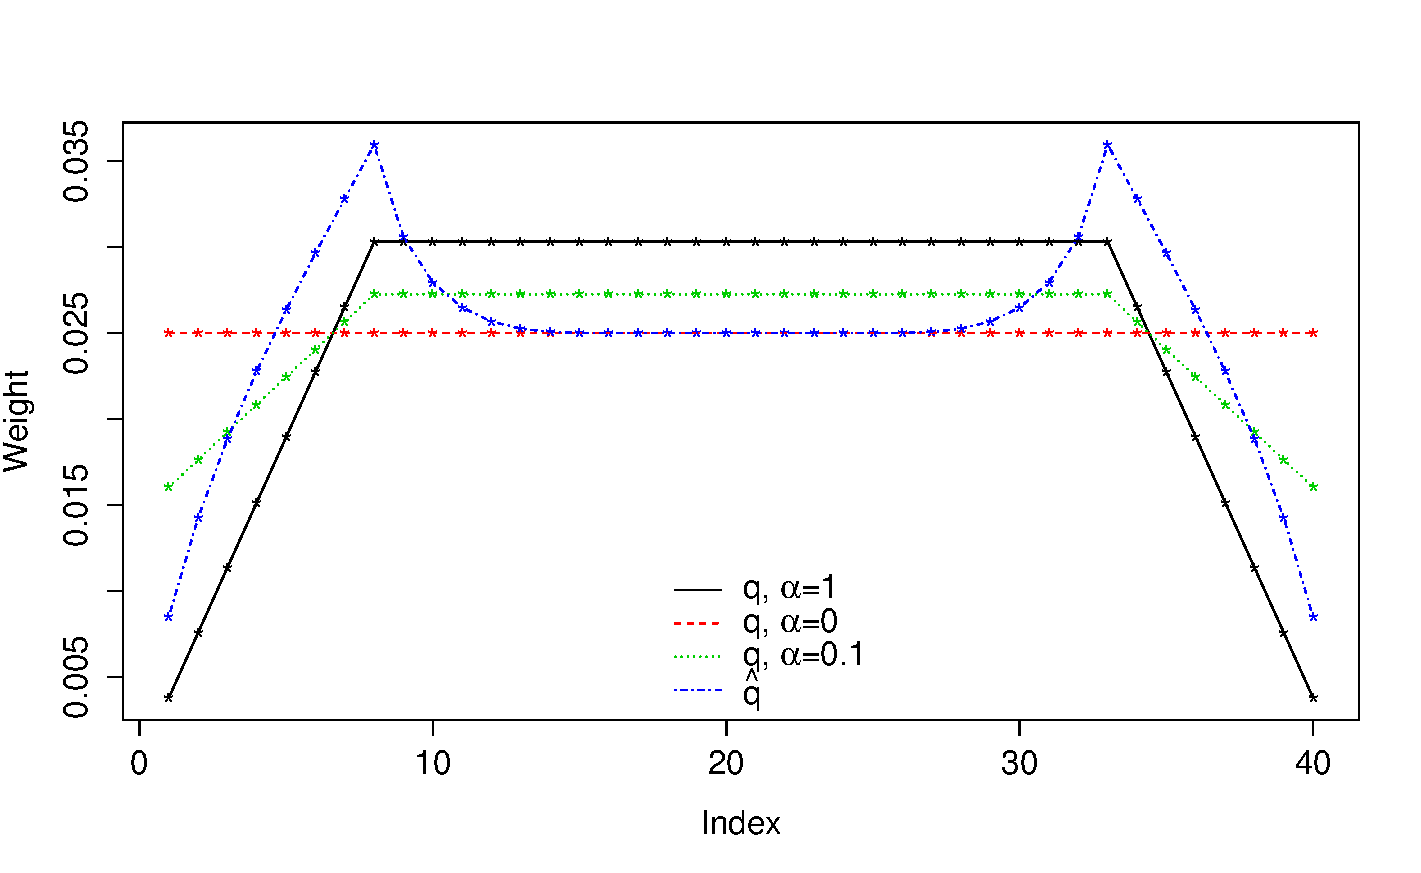
\includegraphics[width = \textwidth]{weights.pdf}\caption{Отнормированные веса ряда $q_i$, соответствующие $\bfC(\alpha)$ и $\widehat\bfC$}\label{img_weights}
\end{center}\end{figure}

\section{Комментарии к алгоритмам. Сравнение}
\label{sec:comments}
Приведем сравнение и комментарии к следующим методам: Weighted Cadzow (Алгоритм \ref{alg:WCIt}), Extended Cadzow (Алгоритм \ref{alg:ECIt}), Алгоритм Cadzow($\alpha$), $0< \alpha \leq 1$, совпадающий с обычным алгоритмом Cadzow при $\alpha=1$,
и Cadzow-$\widehat\bfC$ (Алгоритм \ref{alg:obliqueCadzow}).
Заметим, что длина окна $L$ является параметром всех рассматриваемых методов.

\begin{itemize}
	\item \textit{Теоретическая сходимость.}
	Теорема \ref{th:converg} дает условия существования подпоследовательности, сходящейся к матрице из $\calM_r \cap \calH$. Эта теорема применима напрямую к Алгоритму \ref{alg:obliqueCadzow} в случае положительности всех весов, и к Алгоритму \ref{alg:WCIt} в предположении, что взвешенная проекция на $\calM_r$ вычисляется без ошибки. Теорему \ref{th:converg} легко расширить на случай Алгоритма \ref{alg:ECIt}, где добавленные значения имеют нулевой вес, если рассматривать последовательность $\bfY_k$ вместо $\widetilde\bfY_k$.

	\item \textit{Сходимость на практике.} Несмотря на то, что теория говорит только о существовании сходящихся подпоследовательностей, сходимость полученных последовательностей имела место во всех рассмотренных примерах.
	
	\item \textit{Сравнение по точности.}
	Алгоритмы итеративные, и сходимость к глобальному минимуму в соответствующей задаче метода наименьших квадратов не обязательно имеет место. По этой причине различные алгоритмы, соответствующие одним и тем же весам, могут вести к разным аппроксимациям. В связи с этим, есть смысл в сравнении алгоритмов по точности аппроксимации.	
	%\item \textit{Comparison by computational cost.}
	%Note that we can compare numbers of iterations providing a given accuracy to compare the methods without inner iterations by computational complexity, since computational costs of one iteration are approximately the same.
	\item \textit{Оценка сигнала и аппроксимация ряда.}
	Предложенные методы могут быть рассмотрены и как аппроксимация заданного ряда рядом конечного ранга, и как взвешенный МНК для оценки сигнала. Заметим, что в общем случае качество аппроксимации может противоречить точности оценки из-за возможной переподгонки.
	\item \textit{Алгоритмы и веса ряда.}
	Методы Weighted Cadzow и Extended Cadzow пытаются решить задачу \eqref{L-rank_task} с равными весами $q_i$. Прочие методы работают с весами различной степени неравномерности.
	\item \textit{Алгоритмы и трудоемкость.}
	Все предложенные методы итеративные. Однако, каждая внешняя итерация методов Weighted Cadzow и Extended Cadzow имеет шаг со внутренними итерациями. Следовательно, эти алгоритмы очень трудоемки. Другие методы не содержат внутренних итераций; кроме того, они имеют примерно равную вычислительную стоимость одной итерации, и их можно сравнить с помощью числа итераций.
	Трудоемкость методов определяется как трудоемкостью одной итерации, так и числом итераций. Очевидно, что требуемое количество итераций определяется скоростью сходимости.
	\item \textit{Быстрая реализация.}
	%There is a very fast implementation of iterations of the Cadzow algorithm suggested in \cite{Korobeynikov2010} and extended in \cite{Golyandina.etal2015}. However, it can be shown that the same implementation approach can be applied to the Cadzow($\alpha$) and Cadzow-$\widehat{\bfC}$ algorithms. Therefore, fast implementations of these algorithms still can be compared by the number of iterations.
	Быстрые реализации алгоритма Cadzow, предложенные в \cite{Korobeynikov2010} и дополненные в \cite{Golyandina.etal2015}, могут быть расширены на случай алгоритмов Cadzow($\alpha$) и Cadzow-$\widehat{\bfC}$ с использованием схожего подхода в реализации, см. приложение \ref{sec:fast}. Таким образом, быстрые реализации этих алгоритмов по-прежнему можно сравнивать по числу итераций.
	
	К тому же была предложена быстрая реализация метода Extended Cadzow.
	\item \textit{Использование одной итерации для оценки сигнала.}
	Одна итерация метода Cadzow --- это хорошо известный метод Singular Spectrum Analysis (SSA), который умеет решать существенно большее число задач, чем сам итеративный метод. Кроме предельного ряда, интересна оценка сигнала и с помощью одной итерации рассмотренных методов. В определенном смысле каждый итеративный метод порождает модификацию SSA. Одна итерация, как правило, не дает оценку сигнала рядом конечного ранга. Однако, она имеет низкую трудоемкость и может давать достаточную точность.
	\item \textit{Разделимость, одна итерация и скорость сходимости.}
	В методе SSA есть понятие разделимости, которое определяет свойство метода (приближенно) находить сигнал по наблюдаемой сумме. Тем самым, разделимость
	тесно связана с точностью первой итерации итеративного метода. В свою очередь, естественно предположить, что точность первой итерации связана со скоростью сходимости метода. Поэтому вопросы разделимости имеют отношение к скорости сходимости итеративных алгоритмов.
	\item \textit{Разделимость и выбор параметров.}
	Связь разделимости с длиной окна $L$ для метода SSA хорошо изучена (см., например, \cite{Golyandina2010}). А именно, оптимальная длина окна близка
	к половине длины ряда. Маленькие длины окна $L$ приводят к плохой разделимости. Можно ожидать, что это справедливо и для остальных алгоритмов. Метод Cadzow($\alpha$) имеет дополнительный параметр $\alpha$. Влияние параметра $\alpha$ в классе алгоритмов
	Cadzow ($\alpha$) на разделимость исследуется в приложении~\ref{sec:app} на примере разделения константы и гармоники. Там показано, что малые значения
	$\alpha$ приводят к плохой разделимости, хотя именно они соответствуют примерно равным весам $q_i$ в задаче \eqref{L-rank_task}.
	\item \textit{Равномерные веса ряда и выбор параметров.}
	Рассмотрим зависимость весов ряда в алгоритме Cadzow($\alpha$) от длины окна $L$ или $\alpha$. Предложение~\ref{prop:zhigconseq} показывает, что более равномерные веса достигаются на малых $L$ и малых $\alpha$. Это как раз тот случай, который ведет к плохой разделимости.
	\item \textit{Равномерные веса ряда и точность оценки сигнала.}
	Таким образом более равномерные веса соответствуют алгоритмам, которые имеют либо трудоемкий шаг итерации с внутренними итерациями, либо медленно сходится. Следовательно, такие алгоритмы имеют большую трудоемкость. Отсутствуют теоретические результаты о поведении точности оценки в зависимости от алгоритмов и их параметров. Тем не менее, численные эксперименты показывают, что наилучшая точность достигается на алгоритмах, которым соответствуют одинаковые или почти одинаковые веса.
    \end{itemize}
	
	\begin{remark}
		\label{rem:adjust}
		 Поправка $\calA$, определенная в разделе~\ref{sec:ts} для улучшения оценок, может быть применена в итоговом оценивании сигнала $\widehat\tsS$ для любого из предложенных алгоритмов. Скалярное произведение, использованное в Замечании~\ref{rem:adj} для определения $\calA$ --- обычное эвклидово скалярное произведение, не зависящее от матрицы весов $\bfM$, используемой в алгоритмах, так как норма $\|\cdot\|$ соответствует задаче \eqref{L-rank_task} с равными весами $q_i$. Назовем алгоритмы, к которым применено $\calA$, \emph{алгоритмами с поправкой}. Например, результат $k$-й итерации метода Cadzow можно записать так: $\widehat\tsS_k = \calT^{-1}(\Pi_\calH \Pi_{\calM_r})^k \calT \tsX$. Тогда результат $k$-й итерации поправленного метода Cadzow это $\widehat\tsS_k^*=\calA(\widehat\tsS_k)$.
	\end{remark}

\chapter{Численные эксперименты}
\label{chapter:simul}
\section{Численное моделирование}
\label{sec:simul}
Для исследования работы предложенных алгоритмов были проведены численные эксперименты. Сравнение было проведено на двух примерах: синус и экспоненциально-модулированный синус. Так как результаты, в целом, аналогичны, приведем только результаты, полученные в случае гармонического ряда.

Был взят сигнал $\tsS = (s_{1}, \ldots, s_N)$ длины $N = 40$ и ранга $r=2$, имеющий вид:
\begin{equation}
\label{eq:signal}
s_{k} = 5\sin{\frac{2 \pi k}{6}}, \quad k = 1, \ldots, N,
\end{equation}
и рассматривался ряд вида $\tsX = \tsS + \tsN$, где $\tsN$ --- гауссовский белый шум с нулевым средним и единичной дисперсией. Точность оценки сигнала $\widehat\tsS$ измерялась с помощью корня из среднего по точкам ряда и по 1000 реализациям ряда среднеквадратического отклонения (СКО) от сигнала $\tsS$. Эту меру будем называть RMSE (root mean-square error) оценки сигнала. Сравнение проводилось на одних и тех же реализациях исходного ряда. Результаты сравнения являются значимыми при уровне значимости 5\%.

Сначала был рассмотрен метод Cadzow-$\widehat\bfC$ и класс методов Cadzow($\alpha$). Эти методы используют косоугольное сингулярное разложение матриц; метод Cadzow($1$) совпадает с обыкновенным методом Cadzow. На Рисунке~\ref{img_cadzowspeed2} показана скорость сходимости для $\alpha = 0.1$ и $\alpha = 1$, и для двух различных длин окон $L$. Значения RMSE изображены по оси $y$, среднее число итераций отложено по оси $x$.

\begin{figure}[!hhh]
	%	\begin{center}
	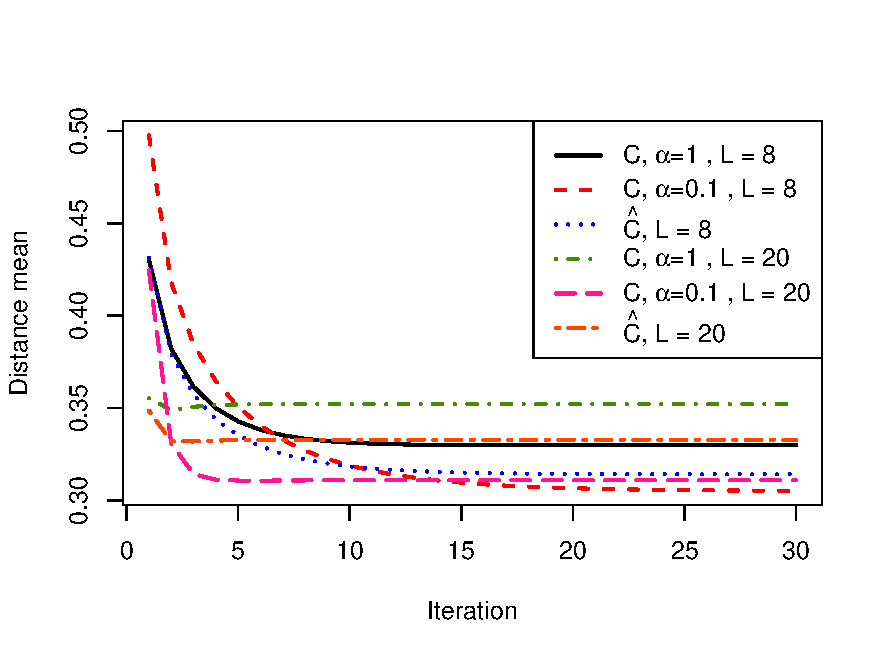
\includegraphics[width = \columnwidth]{cadzowspeed_2.pdf}
	\caption{Зависимость RMSE оценки сигнала от числа итераций, $\sigma = 1$.}
	\label{img_cadzowspeed2}
	%	\end{center}
\end{figure}

Видно, что метод с наименьшей ошибкой в пределе --- тот, который имеет наименьшую скорость сходимости. Среди параметров, использованных для моделирования,  метод Cadzow($0.1$) с длиной окна $L=8$ достиг наименьшей ошибки в пределе. В то же время, эти значения параметров соответствуют как наименьшей скорости сходимости, так и наиболее равномерным весам.

Заметим, что ошибки в пределе сильно не отличаются, они изменяются от 0.31 ($\alpha=0.1$, $L=8$) в лучшем случае до 0.35 ($\alpha=1$, $L=20$) в худшем случае. Тем не менее, ошибка, равная 0.35, достигается на первой итерации в худшем случае, в то время как требуется 4--5 итерации, чтобы достигнуть ошибки 0.35 в лучшем случае.

\smallskip
\begin{figure}[!hhh]
	\begin{center}
	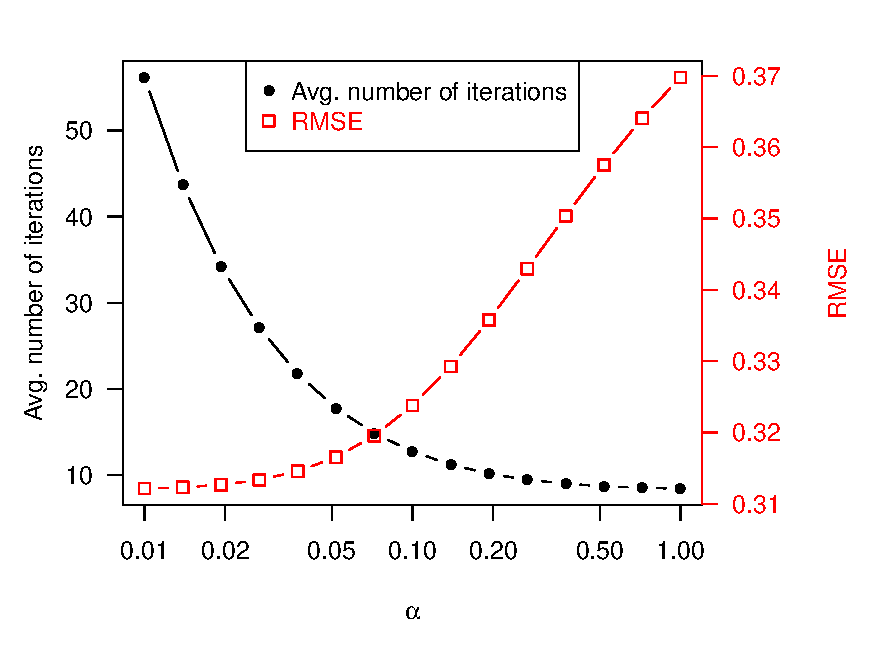
\includegraphics[width = 0.75\columnwidth]{2axis.pdf}
	\caption{RMSE и среднее число итераций в зависимости от $\alpha$ (логарифмическая шкала), $L~=~20$, $\sigma=1$.}
	\label{img_2axis}
	\end{center}
\end{figure}

\begin{figure}[!hhh]
	\begin{center}
	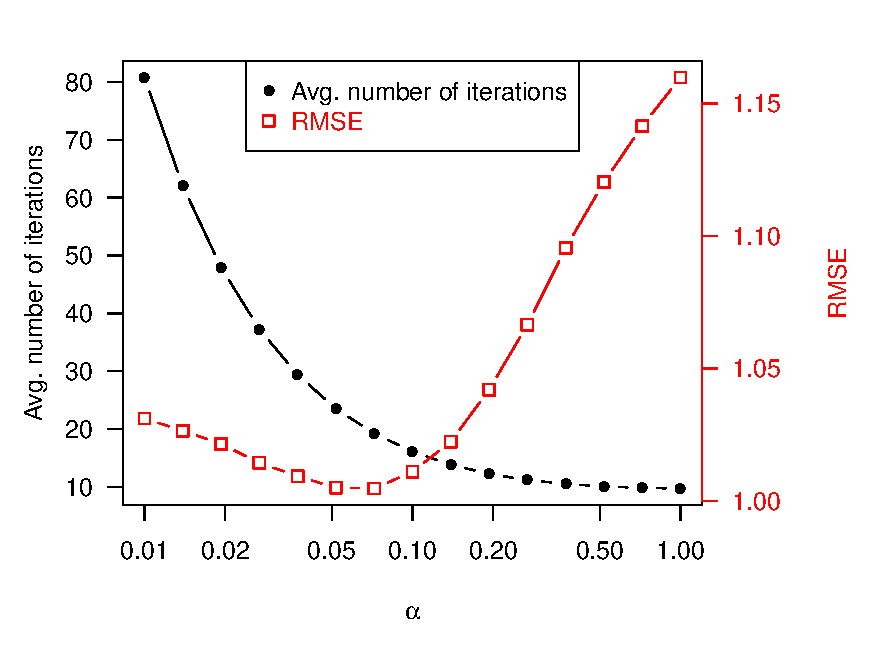
\includegraphics[width = 0.75\columnwidth]{2axis-3.pdf}
	\caption{RMSE и среднее число итераций в зависимости от $\alpha$ (логарифмическая шкала), $L~=~20$, $\sigma=3$.}
	\label{img_2axis-3}
	\end{center}
\end{figure}

Тот же сигнал \eqref{eq:signal} был взят, чтобы понять, как RMSE и скорость сходимости зависят от $\alpha$ для алгоритмов Cadzow($\alpha$). Был использован следующий критерий остановки STOP1: $\frac{\|\calT^{-1}(\bfY_k) - \calT^{-1}(\bfY_{k + 1})\|^2}{N} < 10^{-8}$. Рисунок~\ref{img_2axis} показывает, что меньшие $\alpha$ ведут к лучшим оценкам сигнала, но снижают скорость сходимости алгоритма.

Это общее правило иногда не работает для очень малых значений $\alpha$, см. Рисунок~\ref{img_2axis-3}, где стандартное отклонение шума было увеличено с 1 до 3. Можно увидеть, что для $\alpha$ меньших, чем 0.1, зависимость ошибки оценки от $\alpha$ меняется.
Похоже, что пороговое значение $\alpha$, которое соответствует изменению поведения точности, зависит от разделимости сигнала и шума на одной итерации.
Действительно, можно ожидать,  что для небольших $\alpha$ качество разделимости плохое (см. пример в Приложении).

\smallskip
Включим в рассмотрение методы Extended и Weighted Cadzow, и рассмотрим распределение ошибки восстановления по элементам ряда. В качестве критерия остановки STOP1 было взято число итераций, равное 100 (этот выбор приводит к ошибке, близкой к предельному значению); критерий остановки STOP2 для внутренних итераций выглядит следующим образом:
$\frac{\|\bfY_k - \bfY_{k+1}\|^2}{LK} < 10^{-4}$. Начальные левые и правые продолжения $\tsL_{L-1}$ и $\tsR_{L-1}$ в методе Extended Cadzow были получены при помощи векторного SSA-прогнозирования \cite[глава 2.3.1]{Golyandina.etal2001}.

Рисунки~\ref{fig:s1_it1}~и~\ref{fig:s1_it100} показывают зависимость RMSE от номера точки в ряде. Рисунок~\ref{fig:s1_it1} отображает ошибки на первой итерации, Рисунок~\ref{fig:s1_it100} --- на 100-й итерации. Явно видно, что метод Extended Cadzow наиболее точен в обоих случаях. Методы Cadzow($1$) и Cadzow-$\widehat\bfC$ работают лучше всех на одной итерации среди множества методов без внутренних итераций. Лучший метод в пределе (после 100-й итерации, далее ошибки значительно не изменяются) --- это метод Cadzow($0.1$); это и неудивительно, согласно Рисунку~\ref{img_cadzowspeed2}.

\begin{figure}[!hhh]
	%	\begin{center}
	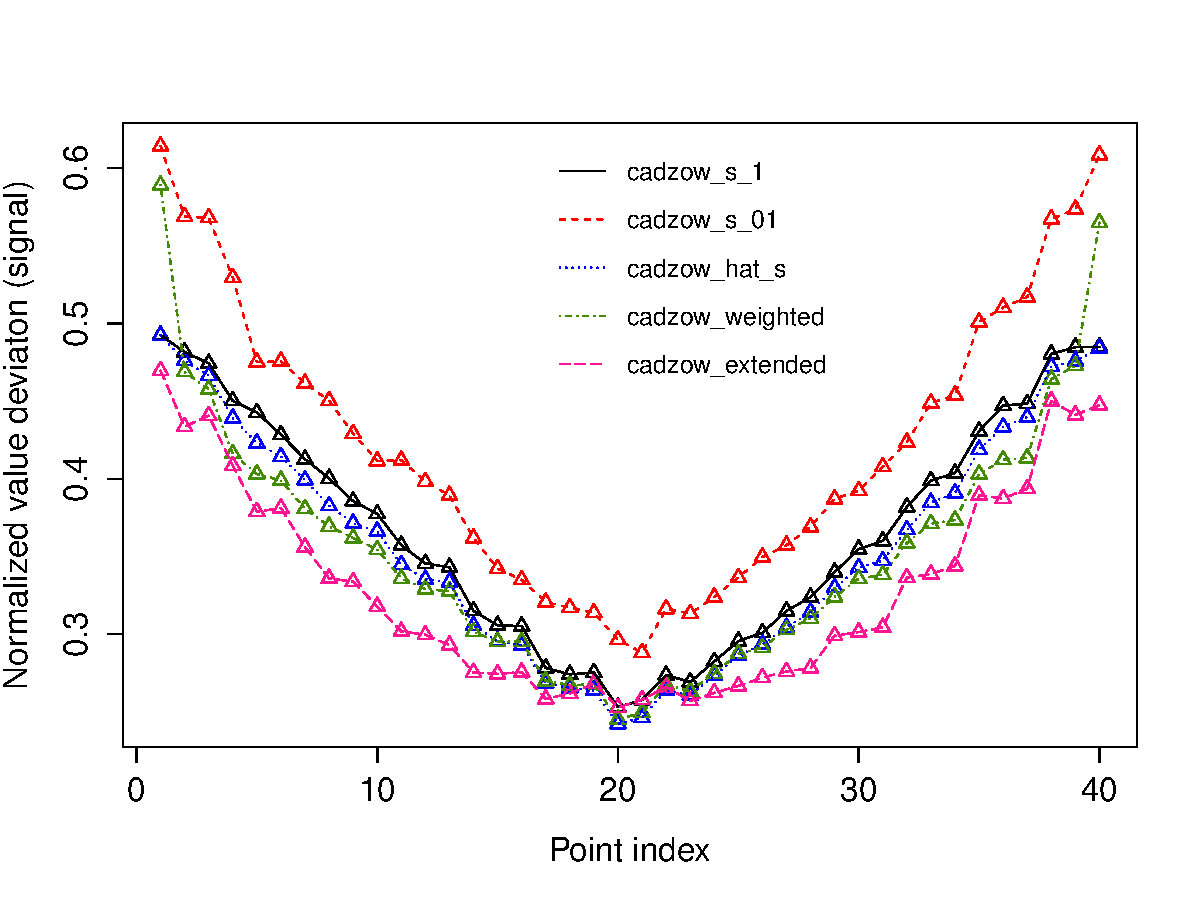
\includegraphics[width = \columnwidth]{s1_it1.pdf}
	\caption{RMSE оценки сигнала на каждой точке ряда; одна итерация; $L=20$, $\sigma=1$.}
	\label{fig:s1_it1}
	%	\end{center}
\end{figure}

\begin{figure}[!hhh]
	%	\begin{center}
	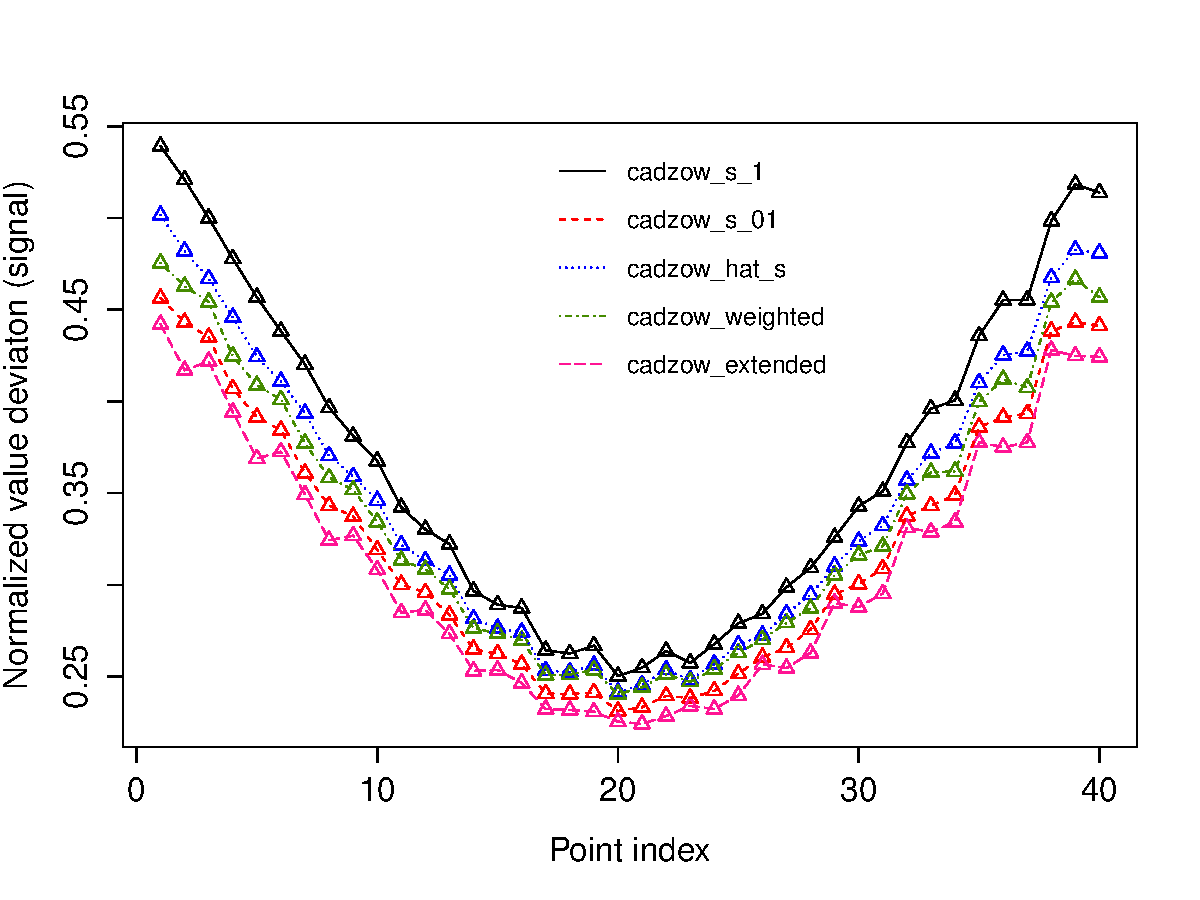
\includegraphics[width = \columnwidth]{s1_it100.pdf}
	\caption{RMSE оценки сигнала на каждой точке ряда; сто итераций; $L=20$, $\sigma=1$.}
	\label{fig:s1_it100}
	%	\end{center}
\end{figure}

\smallskip
Так как был рассмотрен метод наименьших квадратов для оценки сигнала
$\tsS$, приведем Таблицу~\ref{fintable}, которая показывает RMSE для $\tilde \tsS$ как оценки $\tsS$ (то есть ошибку оценки сигнала), и RMSE для $\tilde \tsS$ как оценку начального ряда $\tsX$ (то есть ошибку аппроксимации ряда). Под $k$ обозначено число итераций, $L=20$. Таблица~\ref{fintable} подтверждает заключения о сравнении методов по точности оценки сигнала. Также можно увидеть, что качество аппроксимации начального ряда не всегда соответствуют качеству оценки сигнала. Например, в методе Cadzow($0.1$) на одной итерации явно присутствует переподгонка. Тем не менее, методы одинаково упорядочены по ошибке аппроксимации ряда и оценке сигнала в пределе. Это означает, что, похоже, минимизация ошибки аппроксимации влечет минимизацию ошибки восстановления сигнала.
Это предположение очень важно на практике, так как на реальных примерах можно выбрать наилучшие методы и их параметры, уменьшая ошибку аппроксимации.
Безусловно, необходимо выбрать правильный ранг ряда перед сравнением методов.

Такое же моделирование было проведено для алгоритмов с поправкой (см. Замечание~\ref{rem:adjust}). В Таблице~\ref{fintable_improved} можно увидеть, что точность методов примерно та же. Согласно своему определению, поправка всегда улучшает аппроксимацию изначального ряда; тем не менее, влияние поправки на точность оценки сигнала неоднозначно (поправка улучшает точность на 100-й итерации; результаты различаются на одной итерации).

\begin{table}[!hhh]
	\caption{Сравнение методов по RMSE, $L = 20$, $\sigma=1$.}\label{fintable}
	\begin{center}
	    \begin{tabular}{|c|c|c|c|c|}
    		\hline
    		Метод: & $\tsS$, $k = 1$ & $\tsX$, $k = 1$ & $\tsS$, $k = 100$ & $\tsX$, $k = 100$  \\
		    \hline
		    Cadzow, $\alpha = 1$ & 0.3758 & 0.9195 & 0.3782 & 0.9664 \\
		    \hline
		    Cadzow, $\alpha = 0.1$ & 0.4329 & 0.7040 & 0.3311 & 0.9506 \\
		    \hline
		    Cadzow $\hat{\bfC}$ & 0.3655 & 0.8925 & 0.3559 & 0.9583 \\
		    \hline
		    Weighted Cadzow & 0.3644 & 0.8891 & 0.3455 & 0.9549 \\
		    \hline
		    Extended Cadzow & 0.3361 & 0.9030 & 0.3189 & 0.9471 \\
		    \hline
	    \end{tabular}
	\end{center}
\end{table}

\begin{table}[!hhh]
	\begin{center}
		\caption{Сравнение методов c поправкой по RMSE, $L = 20$, $\sigma=1$.}\label{fintable_improved}
		\begin{tabular}{|c|c|c|c|c|}
			\hline
			Метод: & $\tsS$, $k = 1$ & $\tsX$, $k = 1$ & $\tsS$, $k = 100$ & $\tsX$, $k = 100$  \\
			\hline
			Cadzow, $\alpha = 1$ & 0.3714 & 0.9175 & 0.3667 & 0.9622 \\
			\hline
			Cadzow, $\alpha = 0.1$ & 0.4385 & 0.7023 & 0.3276 & 0.9493 \\
			\hline
			Cadzow $\hat{\bfC}$ & 0.3626 & 0.8909 & 0.3478 & 0.9555 \\
			\hline
			Weighted Cadzow & 0.3640 & 0.8883 & 0.3380 & 0.9523 \\
			\hline
			Extended Cadzow & 0.3370 & 0.9030 & 0.3184 & 0.9469 \\
			\hline
		\end{tabular}
	\end{center}
\end{table}

Таким образом, численные примеры по большей части подтверждают гипотезы и заключения, перечисленные в разделе~\ref{sec:comments}.

\section{Реальный пример}
\label{sec:ex_real}
Был рассмотрен ряд `Fortified wine' (продажи крепленых вин в Австралии, помесячно, с Января 1980 г. по Декабрь 1993 г.) \citep{HyndmanTSDL}. У этого ряда следующая структура: сигнал, состоящий из экспоненциального тренда, сезонная компонента сложной формы и шум.
Было произведено сравнение алгоритмов Cadzow($\alpha$) на различных $\alpha$ и продемонстрировано то, что меньшие $\alpha$ дают меньшую ошибку аппроксимации ряда.

В разделе~\ref{sec:simul} был рассмотрен простой пример сигнала, состоящего из одной синусоиды.
Рассмотренный реальный пример имеет куда более сложную форму. Чтобы подтвердить предположение о том, что можно минимизировать ошибки аппроксимации с целью уменьшения ошибок оценки сигнала,
была построена модель ряда `Fortified wine', и эта модель была использована для моделирования.


Ряд `Fortified wine' был проанализирован в нескольких работах (см., например, \cite{Golyandina.etal2015} для чуть более длинного ряда). Типичный анализ временного ряда основным методом SSA с длиной окна $L=84$ показывает, что ведущие 11 собственных троек
принадлежат сигналу. Метод ESPRIT~\cite{Roy.Kailath1989,Golyandina.Zhigljavsky2012}, примененный к найденному подпространству сигнала, дает оценки основаниям экспоненты $\rho_m$ для тренда и для сезонных компонент, где $k-$й элемент в $m$-й компоненте задан в виде $C_m \rho_m^k$ или $C_m \rho_m^k \sin(2\pi\omega_m k +\phi_m)$, $k=1,\ldots,N$. Метод ESPRIT также оценивает частоты $\omega_m$; тем не менее, для сезонных компонент возможные частоты известны, и поэтому мы изменили оценки сигнала к ближайшим значениям вида $j/12$. Коэффициенты $C_m$ найденных компонент ряда и фазы $\phi_m$ сезонных компонент были оценены по методу наименьших квадратов. Был выбран мультипликативный шум, то есть его стандартное отклонение возрастает пропорционально тренду.
Таким образом, модель сигнала $\tsS = (s_{1}, \ldots, s_N)$, $N=168$, была оценена следующим образом:
%
%%We truncate the series by the first 168 steps,
%We build the parametric form using SSA framework with nested O-SSA iterations \cite{Golyandina2013a} and ESPRIT, estimate the RMSE for various Cadzow($\alpha$), and apply methods to the actual series.
%
%The theoretical signal $\tsS$ was estimated by applying SSA technique to the actual series $\tsX^*$. Let $\tsS = (s_{1}, \ldots, s_N)$ have the length $N = 168$, rank $r=11$, and the form:
\begin{multline*}
s_{k} = 3997.74\, (0.9967)^k + \\
1174.75\, (0.9942)^k \sin(\frac{\pi k}{6} - 2.249) + \\
425.75\, (1.0001)^k \sin(\frac{\pi k}{2} + 2.333) + \\
211.55\, (1.004)^k \sin(\frac{\pi k}{3} + 1.677) + \\
169.33\, (1.0007)^k \sin(\frac{5 \pi k}{6} + 1.533) + \\
361.07\, (0.9884)^k \sin(\frac{2 \pi k}{3} - 2.901).
\end{multline*}
Модель полного ряда следующая: $\tsX=(x_1,\ldots,x_N)$, $x_i=s_i + 353.17 (0.9967)^k \ve_i$,
%where and the series $\tsX = \tsS + \tsU \odot \tsN$ be observed,
где  $\ve_i$, $i=1,\ldots,N$ --- гауссовский белый шум с нулевым средним и единичной дисперсией.
%, $\odot$ is element-wise vector product, $\tsU = (u_{1}, \ldots, u_N)$, $u_k = 353.17 (0.9967)^k$.
%Note that the noise is actually modulated gaussian white noise.
Была выбрана длина окна $L=84$, и применен алгоритм Cadzow($\alpha$) с $\alpha=1$, $0.8$, $0.6$, $0.4$, $0.2$, $0.1$, $0.05$.
Был использован следующий критерий остановки STOP1 в Алгоритме~\ref{alg:obliqueCadzow}:
$\frac{\|\calT^{-1}(\bfY_k) - \calT^{-1}(\bfY_{k + 1})\|^2}{N} <10^{-4}$.
Алгоритм был применен к 1000 независимым реализациям модельного ряда, и к исходному ряду `Fortified wine'.
Таблица~\ref{tab:rltable} содержит RMSE оценки модельного сигнала (колонка $\tsS$),
RMSE аппроксимации модельного ряда (колонка $\tsX$) и точность аппроксимации ряда
`Fortified wines' (колонка $\tsX^*$).

%Accuracy of a signal estimate $\widehat\tsS$ by Cadzow($\alpha$)
%is measured as the root mean-square error (RMSE) using 1000 simulations.
%
%
%Consider Table~\ref{rltable} which shows RMSE for $\tilde \tsS$ as an estimate of $\tsS$ (i.e., signal estimation error), RMSE for $\tilde \tsS$ as an estimate of the initial series $\tsX$ (i.e., series approximation error), and distance to the actual $\tsX^*$ series.

\begin{table}[!hhh]
	\begin{center}
	\caption{Сравнение методов по ошибке восстановления сигнала, аппроксимации ряда `Fortified wine' и его промоделированных копий.}
	\label{tab:rltable}
	
    \begin{tabular}{|c|c|c|c|c|}
		\hline
		Метод: & $\tsS$ & $\tsX$ & $\tsX^*$ \\
		\hline
		Cadzow, $\alpha = 1$ & 127.71 & 263.20 & 283.58 \\
		\hline
		Cadzow, $\alpha = 0.8$ & 127.18 & 262.98 & 283.25 \\
		\hline
		Cadzow, $\alpha = 0.6$ & 126.42 & 262.63 & 282.72 \\
		\hline
		Cadzow, $\alpha = 0.4$ & 125.39 & 262.06 & 281.77 \\
		\hline
		Cadzow, $\alpha = 0.2$ & 124.10 & 260.94 & 279.55 \\
		\hline
		Cadzow, $\alpha = 0.1$ & 125.09 & 260.52 & 276.70 \\
		\hline
		Cadzow, $\alpha = 0.05$ & 129.44 & 261.47 & 274.00 \\
		\hline
	\end{tabular}
	\end{center}
\end{table}

Таблица~\ref{tab:rltable} показывает, что для $\alpha$ из промежутка от 1 до 0.2
меньшая ошибка аппроксимации ведет к меньшей ошибке восстановления. Несмотря на это, для меньших $\alpha$ закономерность исчезает. Вполне возможно, что маленькие значения $\alpha$ не дают достаточной разделимости от шума для сходимости по направлению к глобальному минимуму. 

%As we can see, smaller $\alpha$ tends to better approximation of $\tsX^*$ and estimation of signal $\tsS$, but, according to our investigation, only $\alpha = 1$, $0.8$, $0.6$, $0.4$ and $0.2$  can be trusted. If $\alpha = 0.05$, the separability becomes worse, and small signal-to-noise ratio causes far away from global minimum convergence of algorithm.

Рисунок \ref{fig:rl} показывает аппроксимацию исходного ряда `Fortified wine' $\tsX^*$, полученную алгоритмом Cadzow($0.2$). 
Пунктирная линия соответствует исходному ряду, в то время как сплошная показывает оценку сигнала рядом конечного ранга 11.
Ожидается, что это более точная оценка сигнала рядом конечного ранга, чем оценка SSA или результат Cadzow($1$).

\begin{figure}[!hhh]
	%	\begin{center}
	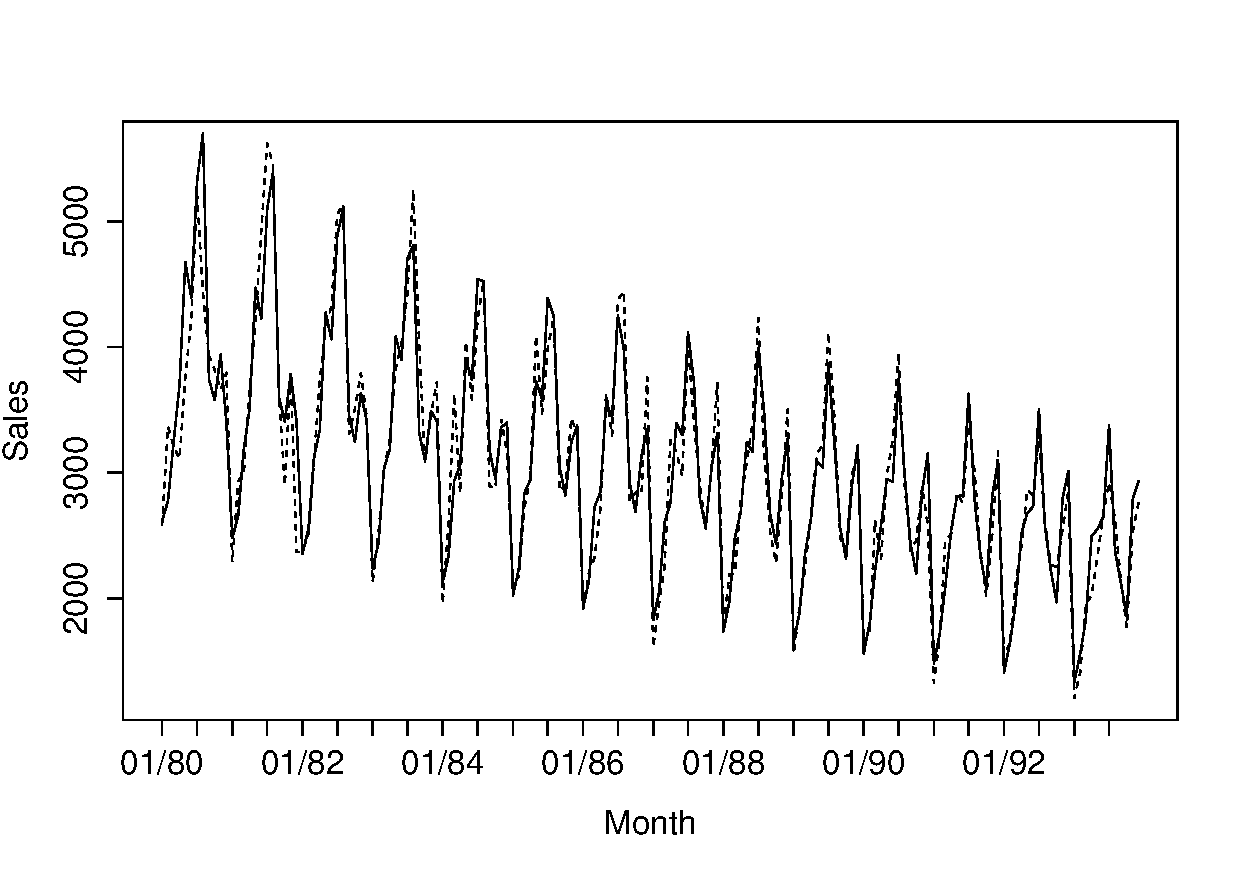
\includegraphics[width=\columnwidth]{rlimage.pdf}
	\caption{Ряд `Fortified wine': применение алгоритма Cadzow($0.2$)}
	\label{fig:rl}
	%	\end{center}
\end{figure}

\conclusion
\label{sec:concl}
В работе были рассмотрены известные итеративные алгоритмы и предложены новые для аппроксимации временного ряда рядами конечного ранга с целью
оценивания сигнала в зашумленном ряде по взвешенному методу наименьших квадратов.

Были рассмотрены эквивалентные постановки задач для взвешенной матричной аппроксимации и взвешенной аппроксимации рядами конечного ранга, где равные веса в задаче МНК для матриц соответствуют неравномерным весам в задаче МНК для временных рядов, и наоборот.

Был рассмотрен довольно широкий набор алгоритмов с целью получить равные веса в МНК. В рассматриваемых алгоритмах равные веса удалось
получить только с помощью алгоритмов со вложенными итерациями, которые сходятся только к локальному экстремуму и вдобавок делают алгоритм очень трудоемким.
Итеративные методы без вложенных итераций дают только приближенно равные веса.

Для рассматриваемого класса алгоритмов типа алгоритмов Cadzow была доказана сходимость внешних итераций алгоритмов по подпоследовательностям.

На примере зашумленного синуса с помощью моделирования были получены результаты по точности и скорости сходимости предлагаемых алгоритмов. Результаты моделирования подтвердили теоретические результаты. Оказывается, что более равномерные веса ряда ведут  к более трудоемким и одновременно более точным методам в пределе. Моделирование также подтверждает тот факт, что скорость сходимости связана с порядком разделимости. Следовательно, для методов без внутренних итераций существует связь между медленной сходимостью, плохой разделимостью, неточной аппроксимацией на первой итерации и точной аппроксимацией в пределе, и наоборот.

\bibliographystyle{gost705}
\bibliography{zvonarev}

\appendix 
\chapter{Разделимость константы и гармоники для алгоритма Cadzow($\alpha$)}
\label{sec:app}

Рассмотрим модификации метода SSA, порожденные одной итерацией алгоритмов Cadzow($\alpha$), описанных в разделе~\ref{sec:cadzow_alpha}. Скажем, что итеративный метод Cadzow($1$) порождает стандартный базовый метод SSA \cite{Golyandina.etal2001,Golyandina.Zhigljavsky2012}, в то время как в общем случае одна итерация метода Cadzow($\alpha$) может быть рассмотрена как частный случай метода Oblique SSA \cite{Golyandina2013} с обычным евклидовым скалярным произведением в пространстве столбцов и специальным скалярным произведением в пространстве строк.

Отделимость сигнала от остатка в методе SSA глубоко изучена в \cite{Golyandina.etal2001,Golyandina2010}. Отделимость сигнала означает способность метода выделять сигнал. На самом деле, разделимость связана с точностью оценки сигнала, полученного на первой итерации предложенных итеративных алгоритмов. Понятия точной, приближенной и асимптотической (при стремлении длины ряда к бесконечности) разделимости вместе с примерами порядков асимптотической разделимости введены для SSA в \cite{Golyandina.etal2001} и могут быть обобщены на косоугольный случай. Следуя \cite{Golyandina.etal2001}, разделимость будет оценена как косинус угла между $L$- и $K$-векторами вложения сигнала и остатка.

Пусть $\bfC \in \sfR^{K \times K}$ --- симметричная неотрицательно определенная матрица, $\tsX_1$ и $\tsX_2$ ---  два разных временных ряда длины $N$, $\bfX^1$, $\bfX^2$ --- их траекторные матрицы. Тогда \emph{коэффициентом корреляции $i$-го и $j$-го столбца} назовем следующую величину:
\begin{equation}\label{col_corr}
\rho^c_{i,j} = \frac{(X^1_i, X^2_j)}{\|X^1_i\| \|X^2_j\|},
\end{equation}
где $X^k_i$ --- $i$-й столбец матрицы $\bfX^k$, $k = 1, 2$, $(\cdot, \cdot)$ --- евклидово скалярное произведение, $\|\cdot\|$ --- евклидова норма. \emph{Коэффициентом корреляции $i$-й и $j$-й строки} назовем следующую величину:
\begin{equation}\label{row_corr}
\rho^r_{i,j} = \frac{(X^{1,i}, X^{2,j})_\bfC}{\|X^{1,i}\|_\bfC \|X^{2,j}\|_\bfC},
\end{equation}
где $X^{k,i}$ --- $i$-я строчка матрицы $\bfX^k$, $k = 1, 2$, а $(\cdot, \cdot)_\bfC$ --- скалярное произведение с матрицей $\bfC$ в $\sfR^K$, определенная следующим образом: $(X, Y)_\bfC = X \bfC Y^\sfT$, так как $X$, $Y$ --- вектор-строчки, $\| \cdot \|_\bfC$ --- норма, порожденная этим скалярным произведением. Скажем, что ряды $\tsX_1$ и $\tsX_2$ \emph{слабо $\varepsilon$---разделимы}, если
\begin{equation}\label{weak_sep_eq}
\rho = \max\Big(\max_{1 \le i,j \le K}|\rho^c_{i,j}|, \max_{1 \le i,j \le L}|\rho^r_{i,j}|\Big) < \varepsilon.
\end{equation}

Нас будет интересовать порядок $\varepsilon$ при $N\ra \infty$ для различных матриц $\bfC$, где ряды $\tsX_k$, $k=1,2$, состоят из первых $N$ членов бесконечного ряда $\tsX_k^\infty$.

Теория применяется на примере гармонического сигнала и константного остатка. По аналогии с SSA можно ожидать, что скорость асимптотической разделимости с белым гауссовским шумом будет такой же.
Таким образом, пусть
$\tsX_1^\infty = (\cos(2 \pi \omega k), k = 1, 2, \ldots)$ и  $\tsX_2^\infty = (c, c, \ldots)$. Вместо $N \to \infty$, удобно рассматривать $L,K \to \infty$ и брать $N = L + K - 1$. Если $\bfC$ -- единичная матрица, то ответ известен: $\varepsilon$ имеет порядок $1/\min(L,K)$, т.е. скорость разделимости равна $1/N$ для $L$, пропорционального $N$.
Этот результат может быть найден в \cite[глава 6.1]{Golyandina.etal2001}.

\smallskip
В следующем утверждении рассматривается порядок разделимости для алгоритма Cadzow ($\alpha$), введенном в разделе~\ref{sec:cadzow_alpha}.


\begin{remark}
	Далее используются следующие обозначения:
	функция $f \in O(g(n))$ при $n\ra \infty$ если существуют $k>0$ и $n_0>0$ такие, что для любых $n > n_0$ выполняется неравенство $|f(n)| \le k |g(n)|$;
	функция $f \in \Omega(g(n))$ при $n\ra \infty$ если существуют $k>0$ и $n_0>0$ такие, что для любых $n > n_0$ выполняется неравенство $|f(n)| \ge k |g(n)|$.
\end{remark}


\begin{proposition}
	\label{prop:separ1}
	Пусть $\tsX_1^\infty = (\cos(2 \pi \omega k), k = 1, 2, \ldots)$, где $0<\omega <0.5$ --- гармонический ряд, $\tsX_2^\infty = (c, c, \ldots)$ --- константный ряд,  $L(N),K(N)\ra \infty$, где $N=L+K-1$, $h = h_N = \lfloor N/L \rfloor$. Пусть также $0<\alpha=\alpha(N)\le 1$ и $\bfC=\bfC(\alpha)$, определенная в \eqref{zhigweights}, т.е. $\bfC$ диагональная матрица с диагональными элементами:
	\begin{equation*}
	c_k = \begin{cases}
	1, & \text{если} \quad k = jL+1 \quad \text{для некоторых} \ j = 0, \ldots, h-1,\\
	\alpha, & \text{в противном случае}.
	\end{cases}
	\end{equation*}
	Тогда
	\begin{enumerate}
		\item $\rho$, заданное в \eqref{weak_sep_eq}, имеет следующий порядок: $\rho~=~O\left(\max\left(\frac{1}{L}, \frac{(1-\alpha)C_{L,K}+\alpha}{(1-\alpha)D_{L,K}+\alpha K}\right)\right)$, где
		\begin{equation*}
		C_{L,K} = C_{L(N),K(N)} = \max_{\substack{1 \le j \le L}}  \sum_{\substack{1 \le k \le K: \\ c_k = 1}}\cos(2 \pi \omega (j + k - 1)),		\end{equation*} и
		\begin{equation*}
		D_{L,K} = D_{L(N),K(N)} = \min_{\substack{1 \le j \le L}} \sum_{\substack{1 \le k \le K: \\ c_k = 1}}\cos^2(2 \pi \omega (j + k - 1)).
		\end{equation*}
		\item Если $h_N$ ограничены константой, то $\rho~=~O\left(\max\left(\frac{1}{L}, \frac{1}{\alpha K}\right)\right)$.
		\item Если существует маленькая $\delta$, $0 < \delta < 1/2$, такая, что $2\,L(N)\,\omega~\in~ \sfR \setminus \left(\bigcup_{k \in \sfZ} [k - \delta, k + \delta] \right)$ для каждой $N$, где $\sfZ$ --- множество целых чисел, то $\rho = O\left(\max\left(\frac{1}{L}, \frac{1}{(1-\alpha)N/L+\alpha K}\right)\right)$.
	\end{enumerate}
	
\end{proposition}

\begin{proof}
	1. Чтобы доказать теорему, необходимо оценить порядки следующих величин:
	\begin{equation}\label{th5_sep1}
	\rho^c_{i,j} = \frac{\sum_{k=j}^{j + L - 1} \cos(2 \pi \omega k)}{\sqrt{L \left(\sum_{k=j}^{j + L - 1} \cos^2(2 \pi \omega k)\right)}},
	\end{equation}
	\begin{equation}\label{th5_sep2}
	\rho^r_{i,j} = \frac{\sum_{k=1}^K c_k\cos(2 \pi \omega (j + k - 1))}{\sqrt{\left(\sum_{k=1}^K c_k\right) \left(\sum_{k=1}^K c_k\cos^2(2 \pi \omega (j + k - 1))\right)}}.
	\end{equation}
	Следующие тригонометрические равенства верны:
	\begin{equation}
	\label{sumcos}
	\sum_{k=1}^n \cos(ak + b) = \csc(a/2) \sin(an / 2) \cos \left(\frac{an + a + 2b}{2} \right), 
	\end{equation}
	\begin{multline}
	\label{sumsqcos}
	\sum_{k=1}^n \cos^2(ak + b) = \frac{1}{4}(2n + \csc(a) \sin(2an + a + 2b) -\\ - \csc(a)\sin(a + 2b)),
	\end{multline}
	для любых вещественных $a, b$ и натурального $n$.
	Так как ряд $\tsX_1$ не является константным, числитель в \eqref{th5_sep1} имеет порядок $O(1)$, в то время как знаменатель имеет порядок $\Omega(L)$. Следовательно, получаем порядок $1/L$.
	
	Чтобы оценить порядок \eqref{th5_sep2}, рассмотрим сумму по $k$ таким, что $c_k=1$, отдельно:
	\begin{multline*}
	\sum_{k=1}^K c_k\cos(2 \pi \omega (j + k - 1)) = \\ (1-\alpha) \sum_{\substack{1 \le k \le K: \\ c_k = 1}}\cos(2 \pi \omega (j + k - 1)) +\\ +\sum_{1 \le k \le K}\alpha \cos(2 \pi \omega (j + k - 1)) = (1-\alpha)O(C_{L,K}) + \alpha\, O(1),
	\end{multline*}
	\begin{equation*}
	\sum_{k=1}^K c_k = (1-\alpha) h + \alpha K,
	\end{equation*}
	и
	\begin{multline*}
	\sum_{k=1}^K c_k\cos^2(2 \pi \omega (j + k - 1)) = \\ (1-\alpha)\sum_{\substack{1 \le k \le K: \\ c_k = 1}}\cos^2(2 \pi \omega (j + k - 1)) +\\ +\sum_{1 \le k \le K }\alpha \cos^2(2 \pi \omega (j + k - 1)) = (1-\alpha) \Theta(D_{L,K}) + \alpha\, \Theta(K).
	\end{multline*}
	
	2. $C_{L,K}$ это в точности максимум из сумм, каждая из которых состоит из $h$ косинусов, таким образом, абсолютное значение $C_{L,K}$ не превосходит $h$, и, если $h_N$ ограничены константой, тогда $|C_{L,K}|$ ограничено той же константой, следовательно $C_{L,K} = O(1)$.
	
	3. Условие $2\,L(N)\,\omega~\in~ \sfR \setminus \left(\bigcup_{k \in \sfZ} [k - \delta, k + \delta] \right)$ гарантирует, что $|\csc(\pi L(N) \omega)|$ в \eqref{sumcos} для $C_{L,K}$ и $|\csc(2 \pi L(N) \omega)|$ в \eqref{sumsqcos} для $D_{L,K}$ ограничены константой, таким образом, получена оценка сверху для $C_{L,K}$ и оценка снизу для $D_{L,K}$. Следовательно, $C_{L, K}$ имеет порядок $O(1)$, в то время как $D_{L, K}$ имеет порядок $\Omega(N/L)$.
\end{proof}

Предположим, что $L(N)$ выбирается так, что $\rho$ имеет порядок $\max\left(\frac{1}{L}, \frac{1}{(1-\alpha)N/L+\alpha K}\right)$. Тогда оптимальный выбор для $L$ это $L \approx \frac{\alpha(N + 1) + \sqrt{\alpha^2(N+1)^2 + 4N(1  - \alpha^2)}}{2(1 + \alpha)}$.
Следовательно, разделимость имеет тот же порядок $O(1/N)$  для $\alpha(N) \to c$, где $0<c\le 1$ --- некоторая константа (однако, меньшей $c$ соответствует меньший множитель перед $1/N$). В случае сходящегося к нулю $\alpha(N) = O(N^{-\beta})$, порядок разделимости становится равным $O(N^{\beta - 1})$ для $0 \le \beta \le 0.5$, и $O(1/\sqrt{N})$ для $\beta > 0.5$.
%
%Теперь рассмотрим алгоритм Cadzow с $\widehat\bfC$, введенный в разделе~\ref{sec:cadzow_hat}.
%
%\begin{proposition}
%\label{prop:separ2}
%Пусть $\tsX_1 = (c, c, \ldots)$ --- некоторая константа и $\tsX_2 = (\cos(2 \pi \omega k), k = 1, 2, \ldots)$, где $0<\omega <0.5$, $L,K\ra \infty$ и $\bfC$ определена в алгоритме Cadzow с $\widehat\bfC$.
% Тогда $\rho$ имеет порядок $\max \left(1/L, \frac{H_L}{\sqrt{NK}} \right)$ при $L, K \to \infty$, где $H_L$ --- $L$-е гармоническое число.
%\end{proposition}
%
%\begin{proof}
%Необходимо оценить порядки следующих величин:
%\begin{gather*}
%\rho^c_{i,j} = \frac{\sum_{k=j}^{j + L - 1} \cos(2 \pi \omega k)}{\sqrt{L (\sum_{k=j}^{j + L - 1} \cos^2(2 \pi \omega k))}}, \\ \rho^r_{i,j} = \frac{\sum_{k=1}^K \hat c_k\cos(2 \pi \omega (j + k - 1))}{\sqrt{(\sum_{k=1}^K \hat c_k) (\sum_{k=1}^K \hat c_k\cos^2(2 \pi \omega (j + k - 1)))}}.
%\end{gather*}
% Порядок $\rho^c_{i,j}$ уже был получен в доказательстве предложения~\ref{prop:separ1}, поэтому сразу перейдем к $\rho^r_{i,j}$. Рассмотрим корреляцию только первых строчек --- для остальных доказательство будет целиком аналогичным. Рассмотрим числитель $\rho^r_{1,1}$:
%\begin{gather*}
%\sum_{k=1}^K \hat c_k\cos(2 \pi \omega k) = \sum_{k=1}^{L-1} \hat c_k\cos(2 \pi \omega k) + \sum_{k=L}^{K - L + 1} \frac{\cos(2 \pi \omega k)}{L} +\\+ \sum_{k=K - L + 2}^{K} \hat c_k\cos(2 \pi \omega k) = I_1 + I_2 + I_3,
%\end{gather*}
%который разбился на три части. Для $I_2$ справедлива оценка $O(1/L)$, а для $I_3$ доказательство аналогично доказательству для $I_1$:
%\begin{gather*}
%|I_1|=\bigg|\sum_{k=1}^{L-1}\frac{1}{L}\left(\frac{k}{L} + \sum_{j=k}^{L-1} \frac{1}{j} \right) \cos(2 \pi \omega k)\bigg| =\\= \bigg|\sum_{k=1}^{L-1} \frac{k \cos(2 \pi \omega k)}{L^2} +  \frac{1}{L}\sum_{k = 1}^{L-1}\sum_{j = k}^{L-1}\frac{\cos(2 \pi \omega k)}{j}\bigg| \le \\ \le
%\bigg|\sum_{k=1}^{L-1} \frac{k \cos(2 \pi \omega k)}{L^2}\bigg| + \bigg|\frac{1}{L}\sum_{k = 1}^{L-1}\sum_{j = k}^{L-1}\frac{\cos(2 \pi \omega k)}{j}\bigg|.
%\end{gather*}
%Используя тот факт, что
%\begin{gather*}
%\sum_{k=1}^n k \cos(ak + b) = -\frac{1}{4}\csc^2(a/2)(-(n+1)\cos(an+b) + \\ + n\cos(an + a + b) + \cos b),
%\end{gather*}
%получаем:
%\begin{gather*}
%\bigg|\sum_{k=1}^{L-1} \frac{k \cos(2 \pi \omega k)}{L^2}\bigg| = O(1/L), \quad
%\bigg|\frac{1}{L}\sum_{k = 1}^{L-1}\sum_{j = k}^{L-1}\frac{\cos(2 \pi \omega k)}{j}\bigg| = \\ =\bigg|\frac{1}{L}\sum_{j = 1}^{L-1}\sum_{k = 1}^{j}\frac{\cos(2 \pi \omega k)}{j}\bigg| \le \bigg|\frac{1}{L}\sum_{j = 1}^{L-1}\frac{d}{j}\bigg| = O \left(\frac{H_L}{L} \right),
%\end{gather*}
%где $d$ --- некоторая константа. 
%
%Для знаменателя нужно рассмотреть следующие суммы:
%\begin{equation*}
%\sum_{k=1}^K \hat c_k = N / L
%\end{equation*}
%по определению, а следующую составляющую просто оценить снизу:
%\begin{equation*}
%\sum_{k=1}^K \hat c_k\cos^2(2 \pi \omega (j + k - 1)) \ge \sum_{k=1}^K \frac{1}{L}\cos^2(2 \pi \omega (j + k - 1)) = O \left(\frac{K}{L} \right).
%\end{equation*}
%\end{proof}

\chapter{Быстрые реализации методов Oblique Cadzow и Extended Cadzow}
\label{sec:fast}
Приведем некоторые результаты, касающиеся эффективной реализации и трудоемкости одной итерации различных методов с использованием подхода, предложенного в статьях \cite{Korobeynikov2010} и \cite{Golyandina2013a}. Суть подхода состоит в том, что можно использовать алгоритм Ланцоша для вычисления частичного сингулярного разложения траекторной матрицы, см. \cite{Korobeynikov2010}. При этом достаточно уметь умножать траекторную матрицу $\bfX$ и ее транспонированный вариант $\bfX^\rmT$ на вектор, что можно сделать быстро в случае, если $\bfX$ --- ганкелева. В случае алгоритма Oblique Cadzow приходится вычислять косоугольное SVD, которое сводится к обычному SVD, но не ганкелевой матрицы. Однако, как будет показано позже, это не является серьезным препятствием.

Также для реализации требуется быстрое взвешенное диагональное усреднение, модификация которого относительно базового случая не является сложной.

Похожим способом были ускорены и внутренние итерации метода Extended Cadzow, разница состоит лишь в том, что для вычисления SVD там используется представление матрицы в виде суммы двух, одна из которых является ганкелевой, а другая имеет простую структуру.

\section{Сведения о быстром умножении ганкелевых матриц}
Обозначим за $A \odot B$ поэлементное умножение векторов $A, B \in \sfC^N$, $\text{conj}(A)$ --- поэлементное комплексное сопряжение. Тогда для комплексного вектора $X \in \sfC^N$ мы определим его дискретное преобразование Фурье:
\begin{equation}\label{Fourier_transform}
\calF_N(X) = \bfF_N X,
\end{equation}
где $\bfF_N \in \sfC^{N \times N}$ --- матрица преобразования Фурье с элементами $(\bfF_N)_{k,l} = e^{-2 \pi i(k-1)(l-1)/N}$. Обратное преобразование Фурье задается следующим образом:
\begin{equation*}
\calF^{-1}_N(X) = \frac{1}{N}\bfF^*_N X,
\end{equation*}
где $\bfF^*_N$ --- эрмитово сопряжение $\bfF_N$.

\emph{Теплицевым циркулянтом} вектора $X=(x_k),$ $k = 1, \ldots, N$, называется матрица
\begin{equation*}
\bfC_T(X) = \begin{pmatrix}
x_1 & x_N & x_{N-1} & \dots & x_3 & x_2 \\ 
x_2 & x_1 & x_N & \dots & x_4 & x_3 \\ 
\vdots & \vdots & \vdots &  & \vdots & \vdots \\ 
x_{N-1} & x_{N-2} & x_{N-3} & \dots & x_1 & x_N \\ 
x_N & x_{N-1} & x_{N-2} & \dots & x_2 & x_1
\end{pmatrix}.
\end{equation*}

\emph{Ганкелевым циркулянтом} вектора $X=(x_k),$ $k = 1, \ldots, N$, называется матрица
\begin{equation*}
\bfC_H(X) = \begin{pmatrix}
x_1 & x_2 & \dots & x_{N-2} & x_{N-1} & x_N \\ 
x_2 & x_3 & \dots & x_{N-1} & x_N & x_1 \\ 
\vdots & \vdots &  & \vdots  & \vdots & \vdots \\ 
x_{N-1} & x_N & \dots & x_{N-4} & x_{N-3} & x_{N-2} \\ 
x_N & x_1 & \dots & x_{N-3} & x_{N-2} & x_{N-1}
\end{pmatrix}.
\end{equation*}

Хорошо известно \cite{Korobeynikov2010}, что умножение Теплицева циркулянта $\bfC_T(X)$ на вектор $A \in \sfC^N$ может быть подсчитано через дискретное преобразование Фурье:
\begin{equation*}
\bfC_T(X) A = \calF_N^{-1}(\calF_N(X) \odot \calF_N(A)).
\end{equation*}
Аналогичное свойство можно записать и для $\bfC_H(X)$.
\begin{lemma}{\cite{Golyandina2013a}}
	Для $X \in \sfC^N$ и $A \in \sfR^N$ выполняется
	\begin{equation*}
	\bfC_H(X) A = \calF_N^{-1}(\calF_N(X) \odot \text{conj}(\calF_N(A))).
	\end{equation*}
\end{lemma}

Для $\tsX \in \sfR^N$ и $K, L$ таких, что $N = K + L - 1$, ганкелева матрица $\calT(\tsX)$ --- это подматрица $\bfC_H(X)$. Поэтому, умножение $\calT(\tsX)$ на вектор может быть записано в следующем виде:

\begin{algorithm}[Быстрое умножение ганкелевой матрицы на вектор, \cite{Golyandina2013a}]\label{fastprod}
	\textbf{Вход}: $V \in \sfR^K$, $\tsX \in \sfR^N$.
	
	\textbf{Результат}:
	$U = \calT(\tsX) V \in \sfR^L$.
	
	\begin{enumerate}
		\item
		$V' \leftarrow \begin{pmatrix}
		V \\ 
		0_{L - 1}
		\end{pmatrix} $
		\item
		$\widehat V' \leftarrow \calF_N(V')$
		\item
		$\hat X \leftarrow \calF_N(\tsX)$
		\item
		$U' \leftarrow \calF_N^{-1}(\hat X \odot \text{conj}(\widehat V'))$
		\item
		$U \leftarrow (u'_1, \ldots, u'_L)^{\rmT}$
	\end{enumerate}
\end{algorithm}
\begin{remark}
	Для умножения матрицы $\bfX^\rmT = (\calT(\tsX))^\rmT$ на вектор $V \in \sfR^L$ достаточно поменять в алгоритме $L$ и $K$ местами.
\end{remark}

%Рассмотрим матрицу $\bfA \in \sfR^{L \times K}$, ранг которой равен единице. Тогда она может быть представлена в виде $\bfA = U V^T$, где $U \in \sfR^L$, $V \in \sfR^K$. Имея такое представление, мы можем умножить матрицу $\bfA$ на произвольный вектор $W \in \sfR^K$ за время $O(L + K)$ следующим образом:
%\begin{equation*}
%\bfA W = \langle V, W \rangle U.
%\end{equation*}

\section{Быстрое сингулярное разложение матрицы в алгоритме Oblique Cadzow}
Следующий шаг --- обобщение предыдущего алгоритма на более широкий класс матриц. Согласно формуле \eqref{eq:PiMr}, на каждой итерации алгоритма Oblique Cadzow необходимо вычислять сингулярное разложение матрицы $\bfB = \bfY \bfO_\bfC^{\rmT}$. И в случае алгоритма Cadzow($\alpha$), и для Cadzow с $\widehat \bfC$, $\bfC$ --- положительно определенная диагональная матрица с диагональными элементами $(c_1, \ldots, c_K)$, при этом $\bfY = \calT(\tsY)$~--- ганкелева. В качестве $\bfO_\bfC$ можно взять матрицу, равную $\text{diag}(\sqrt{c_1}, \ldots, \sqrt{c_K})$. Тогда, используя ассоциативность матричного умножения, можно записать следующие алгоритмы для умножения матриц $\bfB$ и $\bfB^\rmT$ на вектор:
\begin{algorithm}[Умножение матрицы $\bfB$ на вектор]
	\textbf{Вход}: $V \in \sfR^K$, $\tsY \in \sfR^N$, $O \in \sfR^K$, $O = (\sqrt{c_1}, \ldots, \sqrt{c_K})$.
	
	\textbf{Результат}:
	$U = \calT(\tsY) \bfO_\bfC^{\rmT} V = \bfB V \in \sfR^L$.
	
	\begin{enumerate}
		\item
		$V' \leftarrow V \odot O$
		\item
		$U$ --- результат умножения матрицы $\calT(\tsY)$ на вектор $V'$, используя алгоритм \ref{fastprod}.
	\end{enumerate}
\end{algorithm}

\begin{algorithm}[Умножение матрицы $\bfB^\rmT$ на вектор]
	\textbf{Вход}: $V \in \sfR^L$, $\tsY \in \sfR^N$, $O \in \sfR^K$, $O = (\sqrt{c_1}, \ldots, \sqrt{c_K})$.
	
	\textbf{Результат}:
	$U = (\calT(\tsY) \bfO_\bfC^{\rmT})^\rmT V = \bfO_\bfC \calT(\tsY^{\rmT}) V = \bfB^\rmT V \in \sfR^K$.
	
	\begin{enumerate}
		\item
		$U'$ --- результат умножения матрицы $\calT(\tsY)^\rmT$ на вектор $V$, используя алгоритм \ref{fastprod}.
		\item
		$U \leftarrow U' \odot O$
	\end{enumerate}
\end{algorithm}

Не будем приводить общий вид Алгоритма 1 из \cite{Korobeynikov2010} для получения усеченного сингулярного разложения, потому что описанная в данной работе ситуация, кроме способа умножения матрицы на вектор, ничем не отличается.

После применения Алгоритма 1 из \cite{Korobeynikov2010}, получаем частичное сингулярное разложение $\bfB$: сингулярные числа $\sigma'_i,$ $i = 1, \ldots, r$, левые и правые собственные вектора $U'_1, \ldots, U'_r \in \sfR^L$, $V'_1, \ldots, V'_r \in \sfR^K$. По формуле \eqref{eq:PiMr}, результат проекции может быть записан следующим образом:
\begin{equation*}
\Pi_{\calM_r} \bfY = \left(\sum\limits_{i=1}^r \sigma'_i U'_i V_i'^{\rmT}\right) (\bfO_\bfC^{\rmT})^\dagger.
\end{equation*}
Так как была взята диагональная $\bfO_\bfC$, умножение на псевдообратную матрицу к ней может быть легко сосчитано. Положим
\begin{gather*}
O' = (1/\sqrt{c_1}, \ldots, 1/\sqrt{c_K}), \\
\sigma_i = \sigma'_i, \\
U_i = U'_i, \\
V_i = V'_i \odot O'.
\end{gather*}
В итоге получено необходимое представление проекции в виде суммы матриц ранга, равного единице:
$\Pi_{\calM_r} \bfY = \sigma_i U_i V_i^{\rmT}$.
\section{Быстрое взвешенное диагональное усреднение для матрицы единичного ранга}
Пользуясь тем, что операторы $\Pi_\calH$ и $\calT^{-1}$ являются линейными, достаточно уметь производить диагональное усреднение для матрицы единичного ранга, заданной парой из левого и правого вектора $U$ и $V$, по нужной взвешенной метрике. Необходимо действовать согласно общей формуле \eqref{diag_averag}. Заметим, что в нашем случае $m_{l,k}$ не зависит от $l$, и $m_{l,k} = c_k$ определены в \eqref{zhigweights} для алгоритма Cadzow($\alpha$), а для Cadzow с $\widehat \bfC$ $m_{l,k} = \hat c_k$ рассчитаны в Предложении \ref{myweightstat}. Если же посмотреть на знаменатель \eqref{diag_averag}, то можно заметить, что он равен $q_{i+j-1}$ из Предложения \ref{prop:zhigconseq} для Cadzow($\alpha$), а для Cadzow с $\widehat \bfC$ --- $\hat q_{i+j-1}$ из Предложения \ref{myserweightstat}. Таким образом, за исключением нормировки в знаменателе, диагональное усреднение от базового случая существенно не отличается, и соответствующая модификация базового алгоритма, описанного в \cite{Golyandina2013a}, может быть легко записана.
\begin{algorithm}[Быстрое диагональное усреднение]
	\textbf{Вход}: $U \in \sfR^L$, $V \in \sfR^K$, $C = (c_1, \ldots, c_K) \in \sfR^K$, $Q = (q_1, \ldots, q_N) \in \sfR^N$.
	
	\textbf{Результат}:
	$\tilde \tsX = \calT^{-1}\Pi_\calH(U V^{\rmT})$
	
	\begin{enumerate}
		\item
		$U' \leftarrow \begin{pmatrix}
		U \\ 
		0_{K-1}
		\end{pmatrix} $, $V' \leftarrow \begin{pmatrix}
		V \odot C \\ 
		0_{L-1}
		\end{pmatrix} $
		\item
		$\widehat U' \leftarrow \calF_N(U')$, $\widehat V' \leftarrow \calF_N(V')$
		\item
		$\tilde X' \leftarrow \calF^{-1}_N (\widehat U' \odot \widehat V')$
		\item
		$\tilde x_k \leftarrow \tilde x'_k/q_k$, $k = 1, \ldots, N$.
	\end{enumerate}
\end{algorithm}

Учитывая то, что дискретное преобразование Фурье \eqref{Fourier_transform} может быть рассчитано за $O(N \log N)$, где $N$ --- длина вектора, а также соображения по поводу вычислительной сложности алгоритма сингулярного разложения, описанного в \cite{Korobeynikov2010}, получаем оценку для времени работы одной итерации алгоритма Oblique Cadzow, равную $O(r N \log N)$, где $N$ --- длина ряда, $r$ --- требуемый $L$-ранг ряда.

\section{Быстрая реализация внутренних итераций алгоритма Extended Cadzow}
В этом разделе мы продемонстрируем, как можно быстро реализовать сингулярное разложение внутри Алгоритма \ref{alg:weightedSVD}, если исходная матрица взята из алгоритма Extended Cadzow. На самой первой внешней и внутренней итерации мы рассчитываем сингулярное разложение матрицы $\bfY = \bfY_0 = \calT \widetilde\tsX$, где $\widetilde\tsX=(\tsL_{L-1}, \tsX, \tsR_{L-1})$, $\tsX$ --- исходный ряд, а $\tsL_{L-1}$ и $\tsR_{L-1}$ --- изначальные заполнения слева и справа. Эта матрица является ганкелевой, и мы можем применить технику, описанную в \cite{Korobeynikov2010}, для получения обычного частичного сингулярного разложения. Обозначим его сингулярные числа $\sigma_i^{(0)}$, левые вектора --- $U_i^{(0)} \in \sfR^L$, правые --- $V_i^{(0)} \in \sfR^{N + L - 1}$, $i = 1, \ldots, r$

На $t$-й внутренней итерации, $t = 1, 2, \ldots$, требуется рассчитать сингулярное разложение матрицы 
\begin{equation*}
\bfY'_t = \bfY \odot \bfM + \left(\sum\limits_{i=1}^r \sigma_i^{(t-1)} U_i^{(t-1)} (V_i^{(t-1)})^{\rmT}\right) \odot (\bfU - \bfM),
\end{equation*}
где
\begin{equation*}
\bfU = \begin{pmatrix}
1 & \cdots & 1 \\
\vdots & \ddots & \vdots \\
1 & \cdots & 1
\end{pmatrix}, \quad \bfM = (m_{i, j}), \quad m_{i,j} = \begin{cases}
1 & 1 \le i+j-L \le N, \\
0 & \text{в противном случае.}
\end{cases}
\end{equation*}
Заметим следующее: матрица $\bfY \odot \bfM = \calT(0_{L-1}, \tsX, 0_{L-1})$ является ганкелевой, и для нее уже указан быстрый Алгоритм \ref{fastprod} умножения на вектор. Рассмотрим оставшиеся слагаемые: обозначим $\bfZ^{t}_i = (U_i^{(t-1)} (V_i^{(t-1)})^{\rmT}) \odot (\bfU-\bfM)$. Пусть $U_i^{(t-1)} = (u'^{(i)}_1, \ldots, u'^{(i)}_L)^\rmT$, $V_i^{(t-1)} = (v'^{(i)}_1, \ldots, v'^{(i)}_{N + L - 1})^\rmT$. Тогда матрица $\bfZ^{t}_i \in \sfR^{(N + L - 1) \times L}$ имеет вид
\begin{equation*}
\bfZ^{t}_i = \begin{pmatrix}
u'^{(i)}_1 v'^{(i)}_1 & u'^{(i)}_1 v'^{(i)}_2 & \ldots & u'^{(i)}_1 v'^{(i)}_{L-1} & 0 & \ldots & \ldots & 0\\
u'^{(i)}_2 v'^{(i)}_1 & \ldots  &u'^{(i)}_2 v'^{(i)}_{L-2} & 0 & \ldots & \ldots & 0 & u'^{(i)}_2 v'^{(i)}_{N + L - 1} \\ 
\vdots & \iddots & \iddots & \iddots & \iddots & \iddots & \iddots & \vdots \\ 
u'^{(i)}_{L-1} v'^{(i)}_1 & 0 & \ldots & \ldots & 0 & u'^{(i)}_{L-1} v'^{(i)}_{N + 2} & \ldots & u'^{(i)}_{L-1} v'^{(i)}_{N + L - 1} \\
0 & \ldots & \ldots & 0 & u'^{(i)}_L v'^{(i)}_{N + 1} & u'^{(i)}_L v'^{(i)}_{N + 2} & \ldots & u'^{(i)}_L v'^{(i)}_{N + L - 1} \\
\end{pmatrix}.
\end{equation*}

Используя пропорциональность строк матриц $U_i^{(t-1)} (V_i^{(t-1)})^{\rmT}$, матрицы $\bfZ^{t}_i$ и их транспонированный вариант могут быть быстро умножены на вектор с помощью следующих алгоритмов:
\begin{algorithm}[Умножение матрицы $\bfZ^{t}_i$ на вектор]
	\textbf{Вход}: $A = (a_1, \ldots, a_{N + L - 1}) \in \sfR^{N + L - 1}$, $U \in \sfR^L$, $V \in \sfR^{N + L - 1}$
	
	\textbf{Результат}:
	$B = ((U V^{\rmT}) \odot (\bfU-\bfM)) A \in \sfR^L$.
	
	\begin{enumerate}
		\item
		$b'_1 \leftarrow \sum\limits_{i=1}^{L-1}v_i a_i$
		\item
		$b'_k \leftarrow b'_{k-1} + v_{N + L + 1 - k}a_{N + L + 1 - k} - v_{L + 1 - k}a_{L + 1 - k},$ $k = 2, \ldots, L$
		\item
		$B \leftarrow B' \odot U$
	\end{enumerate}
\end{algorithm}

\begin{algorithm}[Умножение матрицы $(\bfZ^{t}_i)^\rmT$ на вектор]
	\textbf{Вход}: $A = (a_1, \ldots, a_L) \in \sfR^L$, $U \in \sfR^L$, $V \in \sfR^{N + L - 1}$
	
	\textbf{Результат}:
	$B = ((U V^{\rmT}) \odot (\bfU-\bfM))^\rmT A \in \sfR^{N + L - 1}$.
	
	\begin{enumerate}
		\item
		$b'_1 \leftarrow \sum\limits_{i=1}^{L - 1}u_i a_i$
		\item
		$b'_k \leftarrow \begin{cases}
		b'_{k - 1} - u_{L + 1 - k} a_{L + 1 - k}, & k \le L, \\
		b'_{k - 1} + u_{N + L + 1 - k} a_{N + L + 1 - k}, & k \ge N + 1,\\
		0, & \text{в противном случае}
		\end{cases}$, $k = 2, \ldots, N + L - 1$
		\item
		$B \leftarrow B' \odot V$
	\end{enumerate}
\end{algorithm}
Таким образом, матрицы $\bfY'_t$ и $(\bfY'_t)^\rmT$ могут быть умножены за время $O(N \log N + Nr)$, а частичное сингулярное разложение $\sigma_i^{(t)}$, $U_i^{(t)}$, $V_i^{(t)}$, $i = 1, \ldots, r$ может быть получено за время $O(r N \log N + N r^2)$. 
\begin{remark}
	Для практической реализации EM-алгоритма требуется критерий остановки. Чаще всего используется сходимость к себе, то есть необходимо рассчитывать расстояния между $\Pi_{\calM_r} \bfY'_t$ и $\Pi_{\calM_r} \bfY'_{t + 1}$ в соответствующей норме. Эта нетривиальная задача может быть решена с помощью разложения матриц в сумму матриц единичного ранга, после чего требуемые скалярные расстояния могут быть рассчитаны с помощью алгоритмов, подобных описанным выше. Таким образом, критерий остановки может быть вычислен за $O(N r^2)$.
\end{remark}

\end{document}